%% SDCM Step 1 — Flowchart
%% Requires: tikz, amsmath, amssymb
%% TikZ libraries: shapes.geometric, arrows.meta, positioning, fit, backgrounds, calc
%%
%% Standalone usage:
%%   pdflatex sdcm_step1_flowchart.tex
%%
%% Include in existing document:
%%   \begin{figure}[htbp]
%%     \centering
%%     \resizebox{\linewidth}{!}{%% SDCM Step 1 — Flowchart
%% Requires: tikz, amsmath, amssymb
%% TikZ libraries: shapes.geometric, arrows.meta, positioning, fit, backgrounds, calc
%%
%% Standalone usage:
%%   pdflatex sdcm_step1_flowchart.tex
%%
%% Include in existing document:
%%   \begin{figure}[htbp]
%%     \centering
%%     \resizebox{\linewidth}{!}{%% SDCM Step 1 — Flowchart
%% Requires: tikz, amsmath, amssymb
%% TikZ libraries: shapes.geometric, arrows.meta, positioning, fit, backgrounds, calc
%%
%% Standalone usage:
%%   pdflatex sdcm_step1_flowchart.tex
%%
%% Include in existing document:
%%   \begin{figure}[htbp]
%%     \centering
%%     \resizebox{\linewidth}{!}{%% SDCM Step 1 — Flowchart
%% Requires: tikz, amsmath, amssymb
%% TikZ libraries: shapes.geometric, arrows.meta, positioning, fit, backgrounds, calc
%%
%% Standalone usage:
%%   pdflatex sdcm_step1_flowchart.tex
%%
%% Include in existing document:
%%   \begin{figure}[htbp]
%%     \centering
%%     \resizebox{\linewidth}{!}{\input{sdcm_step1_flowchart_body.tex}}
%%     \caption{SDCM Step 1 -- Search Strategy}
%%   \end{figure}
%%
%% ZERO custom \newcommand definitions — safe with any package combination
%% (physics, braket, etc.).  All names are prefixed sdcm@ to avoid clashes.

\documentclass[tikz, border=10pt]{standalone}
\usepackage{tikz}
\usepackage{amsmath, amssymb}
\usetikzlibrary{shapes.geometric, arrows.meta, positioning, fit, backgrounds, calc}

% Colors (hex taken 1:1 from the widget)
\definecolor{sdcm@gray@bg}{RGB}{241,239,232}
\definecolor{sdcm@gray@bd}{RGB}{136,135,128}
\definecolor{sdcm@gray@tx}{RGB}{ 44, 44, 42}
\definecolor{sdcm@teal@bg}{RGB}{225,245,238}
\definecolor{sdcm@teal@bd}{RGB}{ 15,110, 86}
\definecolor{sdcm@teal@tx}{RGB}{  8, 80, 65}
\definecolor{sdcm@purp@bg}{RGB}{238,237,254}
\definecolor{sdcm@purp@bd}{RGB}{ 83, 74,183}
\definecolor{sdcm@purp@tx}{RGB}{ 38, 33, 92}
\definecolor{sdcm@ambr@bg}{RGB}{250,238,218}
\definecolor{sdcm@ambr@bd}{RGB}{133, 79, 11}
\definecolor{sdcm@ambr@tx}{RGB}{ 65, 36,  2}
\definecolor{sdcm@corl@bg}{RGB}{250,236,231}
\definecolor{sdcm@corl@bd}{RGB}{153, 60, 29}
\definecolor{sdcm@corl@tx}{RGB}{ 74, 27, 12}
\definecolor{sdcm@gren@bg}{RGB}{234,243,222}
\definecolor{sdcm@gren@bd}{RGB}{ 59,109, 17}
\definecolor{sdcm@gren@tx}{RGB}{ 23, 52,  4}
\definecolor{sdcm@red@bg} {RGB}{252,235,235}
\definecolor{sdcm@red@bd} {RGB}{163, 45, 45}
\definecolor{sdcm@red@tx} {RGB}{ 80, 19, 19}

% TikZ styles (all prefixed sdcm@ to avoid name clashes)
\tikzset{
  sdcm@base/.style={rectangle, rounded corners=6pt,
    minimum width=11cm, minimum height=0.9cm, text width=10.6cm,
    align=center, font=\small, inner sep=6pt, line width=0.4pt},
  sdcm@gray/.style={sdcm@base,
    fill=sdcm@gray@bg, draw=sdcm@gray@bd, text=sdcm@gray@tx},
  sdcm@teal/.style={sdcm@base,
    fill=sdcm@teal@bg, draw=sdcm@teal@bd, text=sdcm@teal@tx},
  sdcm@purp/.style={sdcm@base,
    fill=sdcm@purp@bg, draw=sdcm@purp@bd, text=sdcm@purp@tx},
  sdcm@ambr/.style={sdcm@base,
    fill=sdcm@ambr@bg, draw=sdcm@ambr@bd, text=sdcm@ambr@tx},
  sdcm@corl/.style={sdcm@base,
    fill=sdcm@corl@bg, draw=sdcm@corl@bd, text=sdcm@corl@tx},
  sdcm@purpsm/.style={rectangle, rounded corners=6pt,
    minimum width=5.2cm, minimum height=0.85cm, text width=4.9cm,
    align=center, font=\small, inner sep=5pt, line width=0.4pt,
    fill=sdcm@purp@bg, draw=sdcm@purp@bd, text=sdcm@purp@tx},
  sdcm@gren/.style={rectangle, rounded corners=6pt,
    minimum width=4.8cm, minimum height=0.85cm, text width=4.5cm,
    align=center, font=\small, inner sep=5pt, line width=0.4pt,
    fill=sdcm@gren@bg, draw=sdcm@gren@bd, text=sdcm@gren@tx},
  sdcm@red/.style={rectangle, rounded corners=6pt,
    minimum width=4.8cm, minimum height=0.85cm, text width=4.5cm,
    align=center, font=\small, inner sep=5pt, line width=0.4pt,
    fill=sdcm@red@bg, draw=sdcm@red@bd, text=sdcm@red@tx},
  sdcm@disc/.style={rectangle, rounded corners=6pt,
    minimum width=4.8cm, minimum height=0.85cm, text width=4.5cm,
    align=center, font=\small, inner sep=5pt, line width=0.4pt,
    fill=sdcm@gray@bg, draw=sdcm@gray@bd, text=sdcm@gray@tx},
  sdcm@loop/.style={rectangle, rounded corners=5pt,
    fill=sdcm@purp@bg, draw=sdcm@purp@bd,
    font=\footnotesize, text=sdcm@purp@bd,
    inner sep=5pt, line width=0.6pt,
    minimum width=10cm, text width=9.6cm, align=center},
  sdcm@arr/.style={-{Stealth[length=5pt,width=4pt]},
    line width=0.8pt, color=sdcm@gray@bd},
  sdcm@line/.style={line width=0.8pt, color=sdcm@gray@bd},
}

\begin{document}
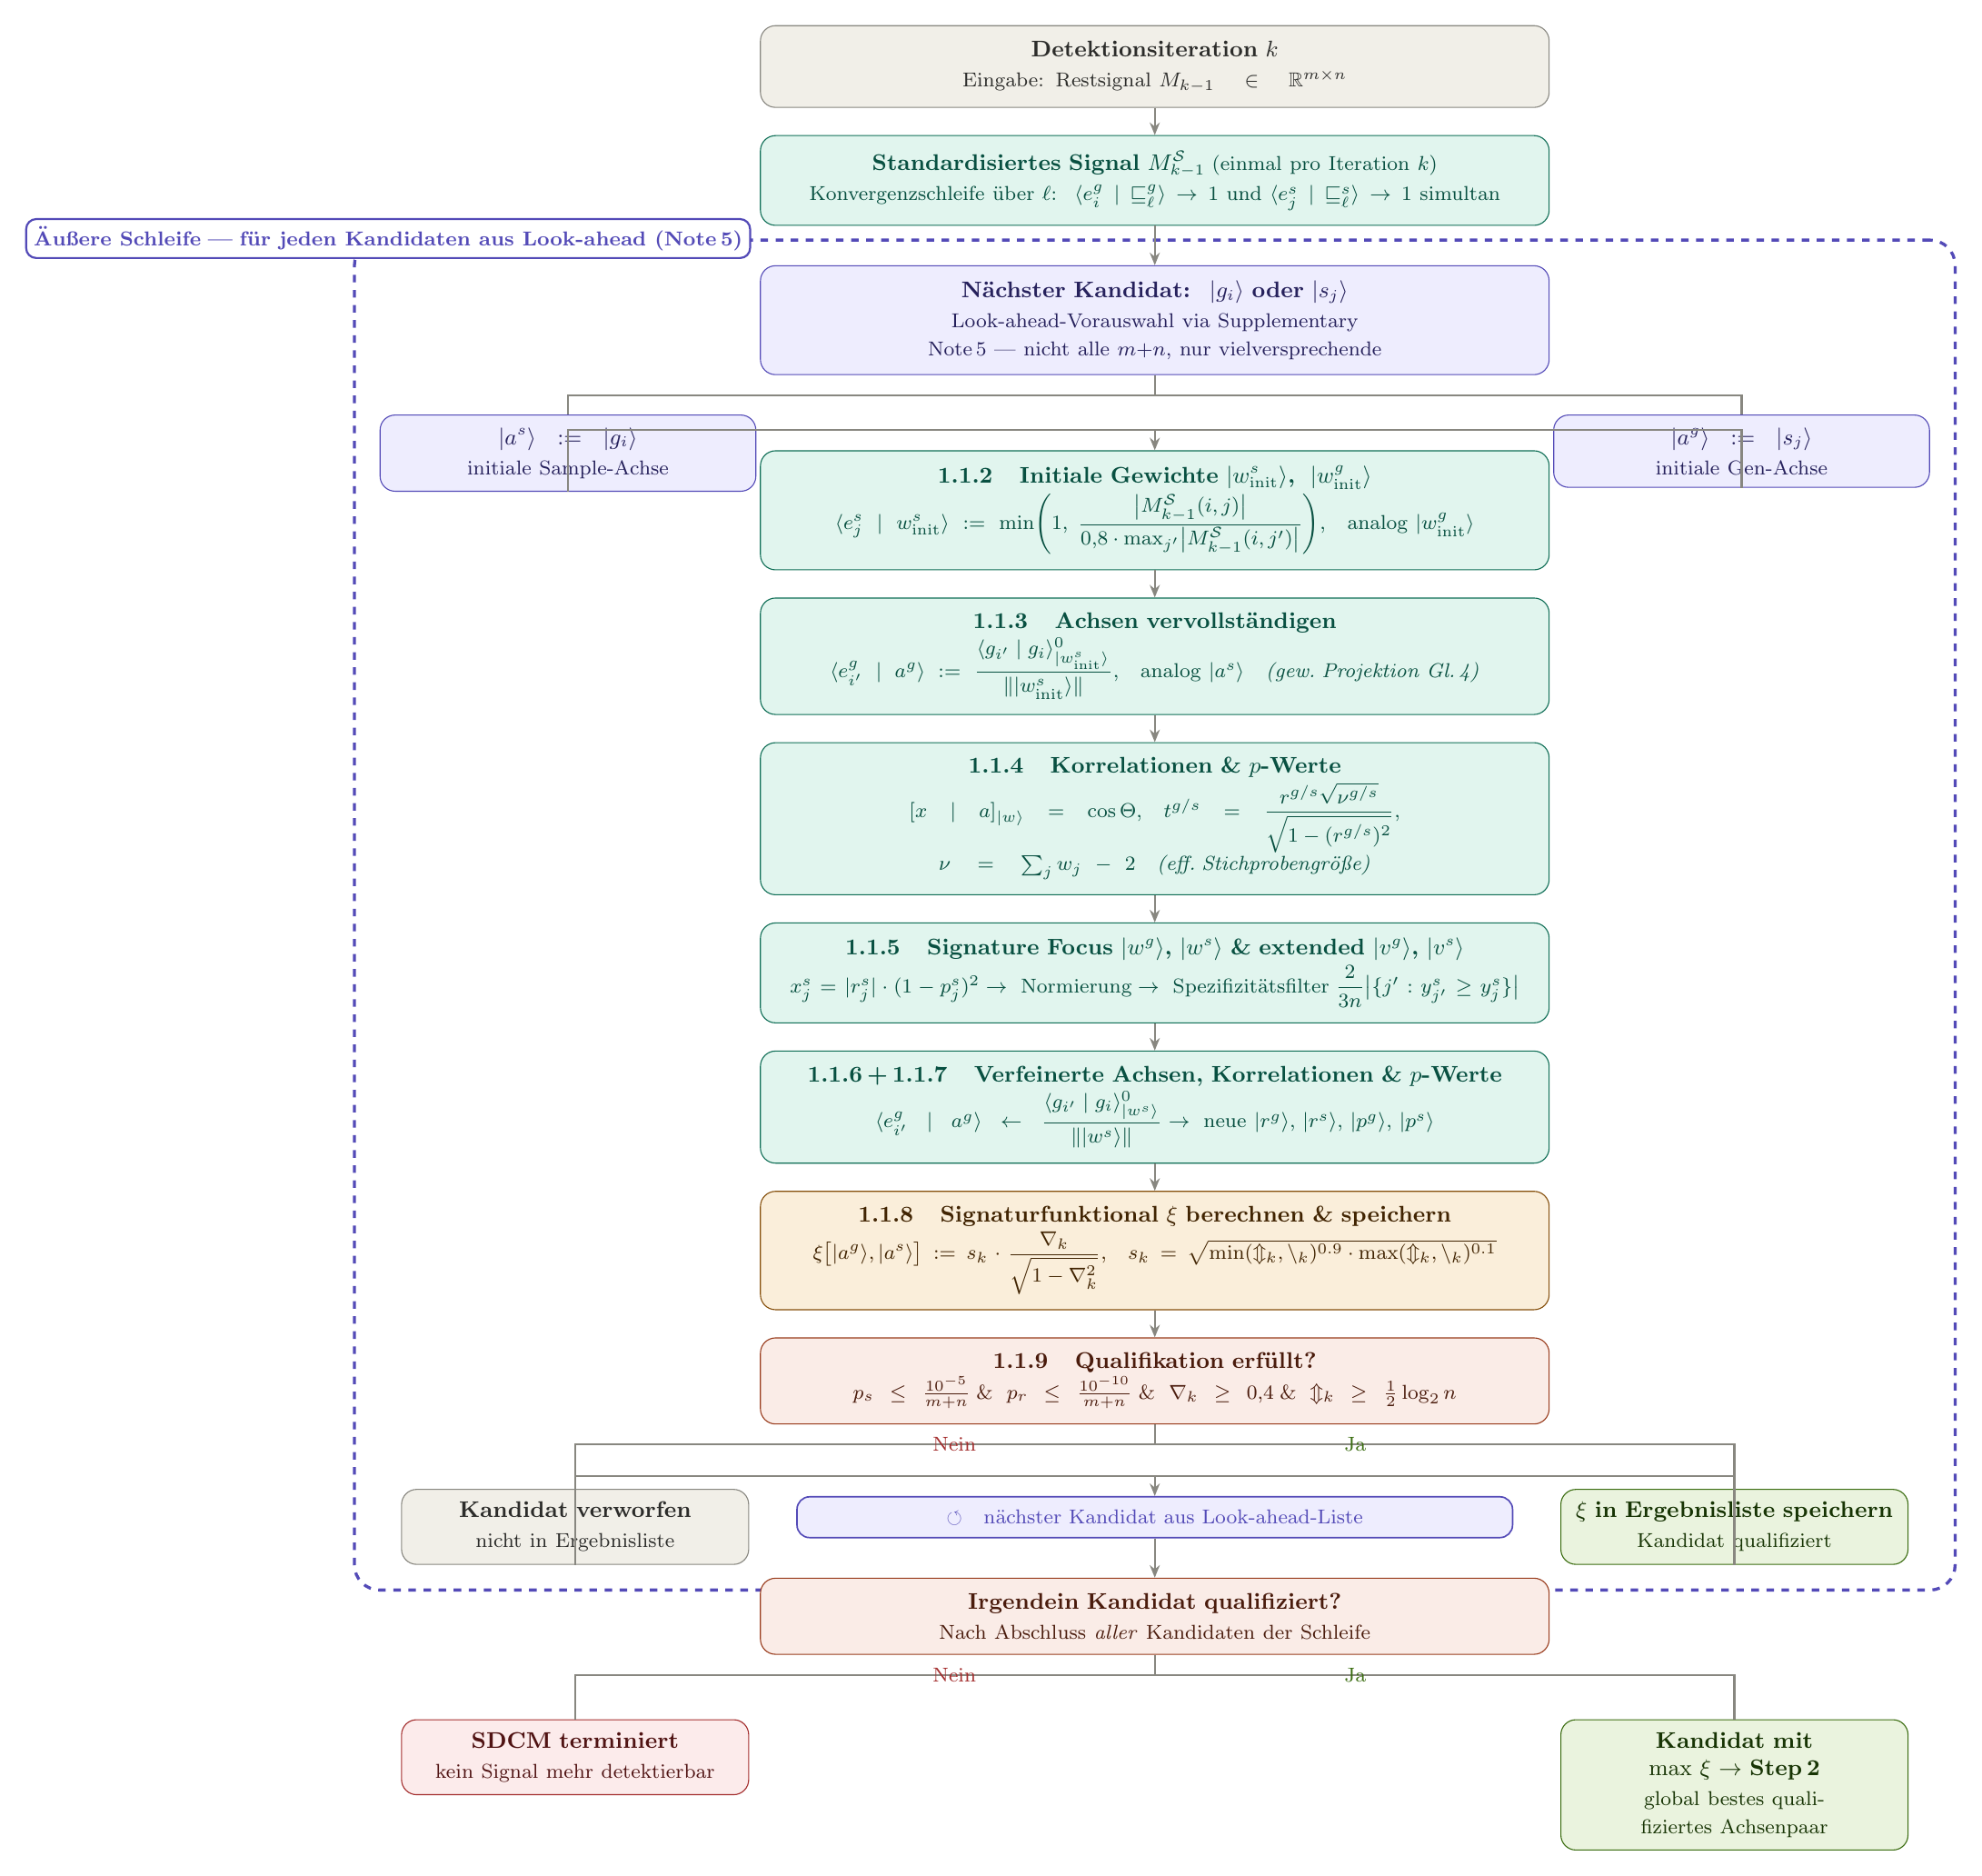
\begin{tikzpicture}[node distance=0.38cm]

% (0) Start
\node[sdcm@gray] (start) {%
  \textbf{Detektionsiteration $k$}\\[1pt]
  {\footnotesize Eingabe: Restsignal $M_{k-1} \in \mathbb{R}^{m \times n}$}%
};

% (1) Standardisierung — once per iteration k, OUTSIDE the loop
\node[sdcm@teal, below=of start] (std) {%
  \textbf{Standardisiertes Signal $M^{\mathcal{S}}_{k-1}$}%
  \;{\footnotesize (einmal pro Iteration $k$)}\\[1pt]
  {\footnotesize Konvergenzschleife über $\ell$:\;
   $\langle e^g_i \mid \mathcal{v}^g_\ell \rangle \to 1$ und
   $\langle e^s_j \mid \mathcal{v}^s_\ell \rangle \to 1$ simultan}%
};

% (2) Candidate — first node inside outer loop
\node[sdcm@purp, below=0.55cm of std] (cand) {%
  \textbf{Nächster Kandidat:\; $|g_i\rangle$ oder $|s_j\rangle$}\\[1pt]
  {\footnotesize Look-ahead-Vorauswahl via Supplementary Note\,5
   — nicht alle $m{+}n$, nur vielversprechende}%
};

% (2a/2b) Branch boxes
\node[sdcm@purpsm, below left=0.55cm and 0.05cm of cand]  (branchL)
  {\textbf{$|a^s\rangle := |g_i\rangle$}\\[1pt]{\footnotesize initiale Sample-Achse}};
\node[sdcm@purpsm, below right=0.55cm and 0.05cm of cand] (branchR)
  {\textbf{$|a^g\rangle := |s_j\rangle$}\\[1pt]{\footnotesize initiale Gen-Achse}};

% (3) Initial weights
\node[sdcm@teal, below=1.05cm of cand] (wini) {%
  \textbf{1.1.2\quad Initiale Gewichte
    $|w^s_\mathrm{init}\rangle$,\; $|w^g_\mathrm{init}\rangle$}\\[1pt]
  {\footnotesize $\displaystyle
    \langle e^s_j \mid w^s_\mathrm{init}\rangle
    := \min\!\left(1,\;
       \frac{\bigl|M^{\mathcal{S}}_{k-1}(i,j)\bigr|}
            {0{,}8\cdot\max_{j'}\bigl|M^{\mathcal{S}}_{k-1}(i,j')\bigr|}
    \right)$,\quad analog $|w^g_\mathrm{init}\rangle$}%
};

% (4) Complete axes
\node[sdcm@teal, below=of wini] (axes) {%
  \textbf{1.1.3\quad Achsen vervollständigen}\\[1pt]
  {\footnotesize $\displaystyle
    \langle e^g_{i'} \mid a^g\rangle
    := \frac{\langle g_{i'} \mid g_i\rangle^0_{|w^s_\mathrm{init}\rangle}}
            {\||w^s_\mathrm{init}\rangle\|}$,\quad
   analog $|a^s\rangle$\quad\textit{(gew.\;Projektion Gl.\,4)}}%
};

% (5) Correlations & p-values
\node[sdcm@teal, below=of axes] (corr) {%
  \textbf{1.1.4\quad Korrelationen \& $p$-Werte}\\[1pt]
  {\footnotesize
   $[x \mid a]_{|w\rangle} = \cos\Theta$,\quad
   $t^{g/s} = \dfrac{r^{g/s}\sqrt{\nu^{g/s}}}{\sqrt{1-(r^{g/s})^2}}$,\quad
   $\nu = \textstyle\sum_j w_j - 2$\quad\textit{(eff.\;Stichprobengröße)}}%
};

% (6) Signature Focus
\node[sdcm@teal, below=of corr] (focus) {%
  \textbf{1.1.5\quad Signature Focus
    $|w^g\rangle$, $|w^s\rangle$ \& extended $|v^g\rangle$, $|v^s\rangle$}\\[1pt]
  {\footnotesize
   $x^s_j = |r^s_j|\cdot(1-p^s_j)^2$\;$\to$\;
   Normierung\;$\to$\;
   Spezifizitätsfilter\;$\dfrac{2}{3n}\bigl|\{j': y^s_{j'}\ge y^s_j\}\bigr|$}%
};

% (7) Refined axes
\node[sdcm@teal, below=of focus] (refit) {%
  \textbf{1.1.6\,+\,1.1.7\quad Verfeinerte Achsen, Korrelationen \& $p$-Werte}\\[1pt]
  {\footnotesize
   $\langle e^g_{i'} \mid a^g\rangle
    \leftarrow \dfrac{\langle g_{i'}\mid g_i\rangle^0_{|w^s\rangle}}
                     {\||w^s\rangle\|}$\;$\to$\;
   neue $|r^g\rangle,\,|r^s\rangle,\,|p^g\rangle,\,|p^s\rangle$}%
};

% (8) Signature functional
\node[sdcm@ambr, below=of refit] (xi) {%
  \textbf{1.1.8\quad Signaturfunktional $\xi$ berechnen \& speichern}\\[1pt]
  {\footnotesize $\displaystyle
    \xi\bigl[|a^g\rangle,|a^s\rangle\bigr]
    := s_k\cdot\frac{\mathcal{r}_k}{\sqrt{1-\mathcal{r}_k^2}}$,\quad
   $s_k=\sqrt{\min(\mathcal{m}_k,\mathcal{n}_k)^{0.9}
               \cdot\max(\mathcal{m}_k,\mathcal{n}_k)^{0.1}}$}%
};

% (9) Qualification
\node[sdcm@corl, below=of xi] (qual) {%
  \textbf{1.1.9\quad Qualifikation erfüllt?}\\[1pt]
  {\footnotesize
   $p_s\le\tfrac{10^{-5}}{m+n}$\;\&\;
   $p_r\le\tfrac{10^{-10}}{m+n}$\;\&\;
   $\mathcal{r}_k\ge0{,}4$\;\&\;
   $\mathcal{m}_k\ge\tfrac{1}{2}\log_2 n$}%
};

% Qualification branch outcomes
\node[sdcm@disc, below left=0.9cm  and 0.15cm of qual] (disc)
  {\textbf{Kandidat verworfen}\\[1pt]{\footnotesize nicht in Ergebnisliste}};
\node[sdcm@gren, below right=0.9cm and 0.15cm of qual] (save)
  {\textbf{$\xi$ in Ergebnisliste speichern}\\[1pt]{\footnotesize Kandidat qualifiziert}};

% Loop-back banner
\node[sdcm@loop, below=1.0cm of qual] (loopback)
  {$\circlearrowleft$\quad nächster Kandidat aus Look-ahead-Liste};

% Final decision (outside loop)
\node[sdcm@corl, below=0.55cm of loopback] (anyq) {%
  \textbf{Irgendein Kandidat qualifiziert?}\\[1pt]
  {\footnotesize Nach Abschluss \emph{aller} Kandidaten der Schleife}%
};

% Final outcomes
\node[sdcm@red,  below left=0.9cm  and 0.15cm of anyq] (term)
  {\textbf{SDCM terminiert}\\[1pt]{\footnotesize kein Signal mehr detektierbar}};
\node[sdcm@gren, below right=0.9cm and 0.15cm of anyq] (step2)
  {\textbf{Kandidat mit $\max\,\xi$ $\to$ Step\,2}\\[1pt]
   {\footnotesize global bestes qualifiziertes Achsenpaar}};

% Outer loop dashed frame
\begin{scope}[on background layer]
  \node[draw=sdcm@purp@bd, line width=1.2pt, dashed, fill=none,
    rounded corners=10pt, inner sep=10pt,
    fit=(cand)(branchL)(branchR)(wini)(axes)(corr)
        (focus)(refit)(xi)(qual)(disc)(save)(loopback)
  ] (outerloop) {};
\end{scope}
\node[fill=white, draw=sdcm@purp@bd, line width=0.8pt, rounded corners=4pt,
  inner sep=3pt, font=\footnotesize\bfseries, text=sdcm@purp@bd
] at (outerloop.north west) [xshift=14pt]
  {Äußere Schleife\;—\;für jeden Kandidaten aus Look-ahead (Note\,5)};

% Arrows
\draw[sdcm@arr]  (start.south) -- (std.north);
\draw[sdcm@arr]  (std.south)   -- (cand.north);

\coordinate (splitPt) at ($(cand.south)+(0,-0.28)$);
\draw[sdcm@line] (cand.south) -- (splitPt);
\draw[sdcm@line] (splitPt) -| (branchL.north);
\draw[sdcm@line] (splitPt) -| (branchR.north);

\coordinate (mergePt) at ($(wini.north)+(0,0.28)$);
\draw[sdcm@line] (branchL.south) |- (mergePt);
\draw[sdcm@line] (branchR.south) |- (mergePt);
\draw[sdcm@arr]  (mergePt) -- (wini.north);

\draw[sdcm@arr] (wini.south)  -- (axes.north);
\draw[sdcm@arr] (axes.south)  -- (corr.north);
\draw[sdcm@arr] (corr.south)  -- (focus.north);
\draw[sdcm@arr] (focus.south) -- (refit.north);
\draw[sdcm@arr] (refit.south) -- (xi.north);
\draw[sdcm@arr] (xi.south)    -- (qual.north);

\coordinate (qSplit) at ($(qual.south)+(0,-0.28)$);
\draw[sdcm@line] (qual.south) -- (qSplit);
\draw[sdcm@line] (qSplit) -| (disc.north);
\draw[sdcm@line] (qSplit) -| (save.north);
\node[font=\footnotesize, text=sdcm@red@bd]  at ($(qSplit)+(-2.8,0)$) {Nein};
\node[font=\footnotesize, text=sdcm@gren@bd] at ($(qSplit)+(+2.8,0)$) {Ja};

\coordinate (lbMerge) at ($(loopback.north)+(0,0.28)$);
\draw[sdcm@line] (disc.south) |- (lbMerge);
\draw[sdcm@line] (save.south) |- (lbMerge);
\draw[sdcm@arr]  (lbMerge)   -- (loopback.north);
\draw[sdcm@arr]  (loopback.south) -- (anyq.north);

\coordinate (aSplit) at ($(anyq.south)+(0,-0.28)$);
\draw[sdcm@line] (anyq.south) -- (aSplit);
\draw[sdcm@line] (aSplit) -| (term.north);
\draw[sdcm@line] (aSplit) -| (step2.north);
\node[font=\footnotesize, text=sdcm@red@bd]  at ($(aSplit)+(-2.8,0)$) {Nein};
\node[font=\footnotesize, text=sdcm@gren@bd] at ($(aSplit)+(+2.8,0)$) {Ja};

\end{tikzpicture}
\end{document}}
%%     \caption{SDCM Step 1 -- Search Strategy}
%%   \end{figure}
%%
%% ZERO custom \newcommand definitions — safe with any package combination
%% (physics, braket, etc.).  All names are prefixed sdcm@ to avoid clashes.

\documentclass[tikz, border=10pt]{standalone}
\usepackage{tikz}
\usepackage{amsmath, amssymb}
\usetikzlibrary{shapes.geometric, arrows.meta, positioning, fit, backgrounds, calc}

% Colors (hex taken 1:1 from the widget)
\definecolor{sdcm@gray@bg}{RGB}{241,239,232}
\definecolor{sdcm@gray@bd}{RGB}{136,135,128}
\definecolor{sdcm@gray@tx}{RGB}{ 44, 44, 42}
\definecolor{sdcm@teal@bg}{RGB}{225,245,238}
\definecolor{sdcm@teal@bd}{RGB}{ 15,110, 86}
\definecolor{sdcm@teal@tx}{RGB}{  8, 80, 65}
\definecolor{sdcm@purp@bg}{RGB}{238,237,254}
\definecolor{sdcm@purp@bd}{RGB}{ 83, 74,183}
\definecolor{sdcm@purp@tx}{RGB}{ 38, 33, 92}
\definecolor{sdcm@ambr@bg}{RGB}{250,238,218}
\definecolor{sdcm@ambr@bd}{RGB}{133, 79, 11}
\definecolor{sdcm@ambr@tx}{RGB}{ 65, 36,  2}
\definecolor{sdcm@corl@bg}{RGB}{250,236,231}
\definecolor{sdcm@corl@bd}{RGB}{153, 60, 29}
\definecolor{sdcm@corl@tx}{RGB}{ 74, 27, 12}
\definecolor{sdcm@gren@bg}{RGB}{234,243,222}
\definecolor{sdcm@gren@bd}{RGB}{ 59,109, 17}
\definecolor{sdcm@gren@tx}{RGB}{ 23, 52,  4}
\definecolor{sdcm@red@bg} {RGB}{252,235,235}
\definecolor{sdcm@red@bd} {RGB}{163, 45, 45}
\definecolor{sdcm@red@tx} {RGB}{ 80, 19, 19}

% TikZ styles (all prefixed sdcm@ to avoid name clashes)
\tikzset{
  sdcm@base/.style={rectangle, rounded corners=6pt,
    minimum width=11cm, minimum height=0.9cm, text width=10.6cm,
    align=center, font=\small, inner sep=6pt, line width=0.4pt},
  sdcm@gray/.style={sdcm@base,
    fill=sdcm@gray@bg, draw=sdcm@gray@bd, text=sdcm@gray@tx},
  sdcm@teal/.style={sdcm@base,
    fill=sdcm@teal@bg, draw=sdcm@teal@bd, text=sdcm@teal@tx},
  sdcm@purp/.style={sdcm@base,
    fill=sdcm@purp@bg, draw=sdcm@purp@bd, text=sdcm@purp@tx},
  sdcm@ambr/.style={sdcm@base,
    fill=sdcm@ambr@bg, draw=sdcm@ambr@bd, text=sdcm@ambr@tx},
  sdcm@corl/.style={sdcm@base,
    fill=sdcm@corl@bg, draw=sdcm@corl@bd, text=sdcm@corl@tx},
  sdcm@purpsm/.style={rectangle, rounded corners=6pt,
    minimum width=5.2cm, minimum height=0.85cm, text width=4.9cm,
    align=center, font=\small, inner sep=5pt, line width=0.4pt,
    fill=sdcm@purp@bg, draw=sdcm@purp@bd, text=sdcm@purp@tx},
  sdcm@gren/.style={rectangle, rounded corners=6pt,
    minimum width=4.8cm, minimum height=0.85cm, text width=4.5cm,
    align=center, font=\small, inner sep=5pt, line width=0.4pt,
    fill=sdcm@gren@bg, draw=sdcm@gren@bd, text=sdcm@gren@tx},
  sdcm@red/.style={rectangle, rounded corners=6pt,
    minimum width=4.8cm, minimum height=0.85cm, text width=4.5cm,
    align=center, font=\small, inner sep=5pt, line width=0.4pt,
    fill=sdcm@red@bg, draw=sdcm@red@bd, text=sdcm@red@tx},
  sdcm@disc/.style={rectangle, rounded corners=6pt,
    minimum width=4.8cm, minimum height=0.85cm, text width=4.5cm,
    align=center, font=\small, inner sep=5pt, line width=0.4pt,
    fill=sdcm@gray@bg, draw=sdcm@gray@bd, text=sdcm@gray@tx},
  sdcm@loop/.style={rectangle, rounded corners=5pt,
    fill=sdcm@purp@bg, draw=sdcm@purp@bd,
    font=\footnotesize, text=sdcm@purp@bd,
    inner sep=5pt, line width=0.6pt,
    minimum width=10cm, text width=9.6cm, align=center},
  sdcm@arr/.style={-{Stealth[length=5pt,width=4pt]},
    line width=0.8pt, color=sdcm@gray@bd},
  sdcm@line/.style={line width=0.8pt, color=sdcm@gray@bd},
}

\begin{document}
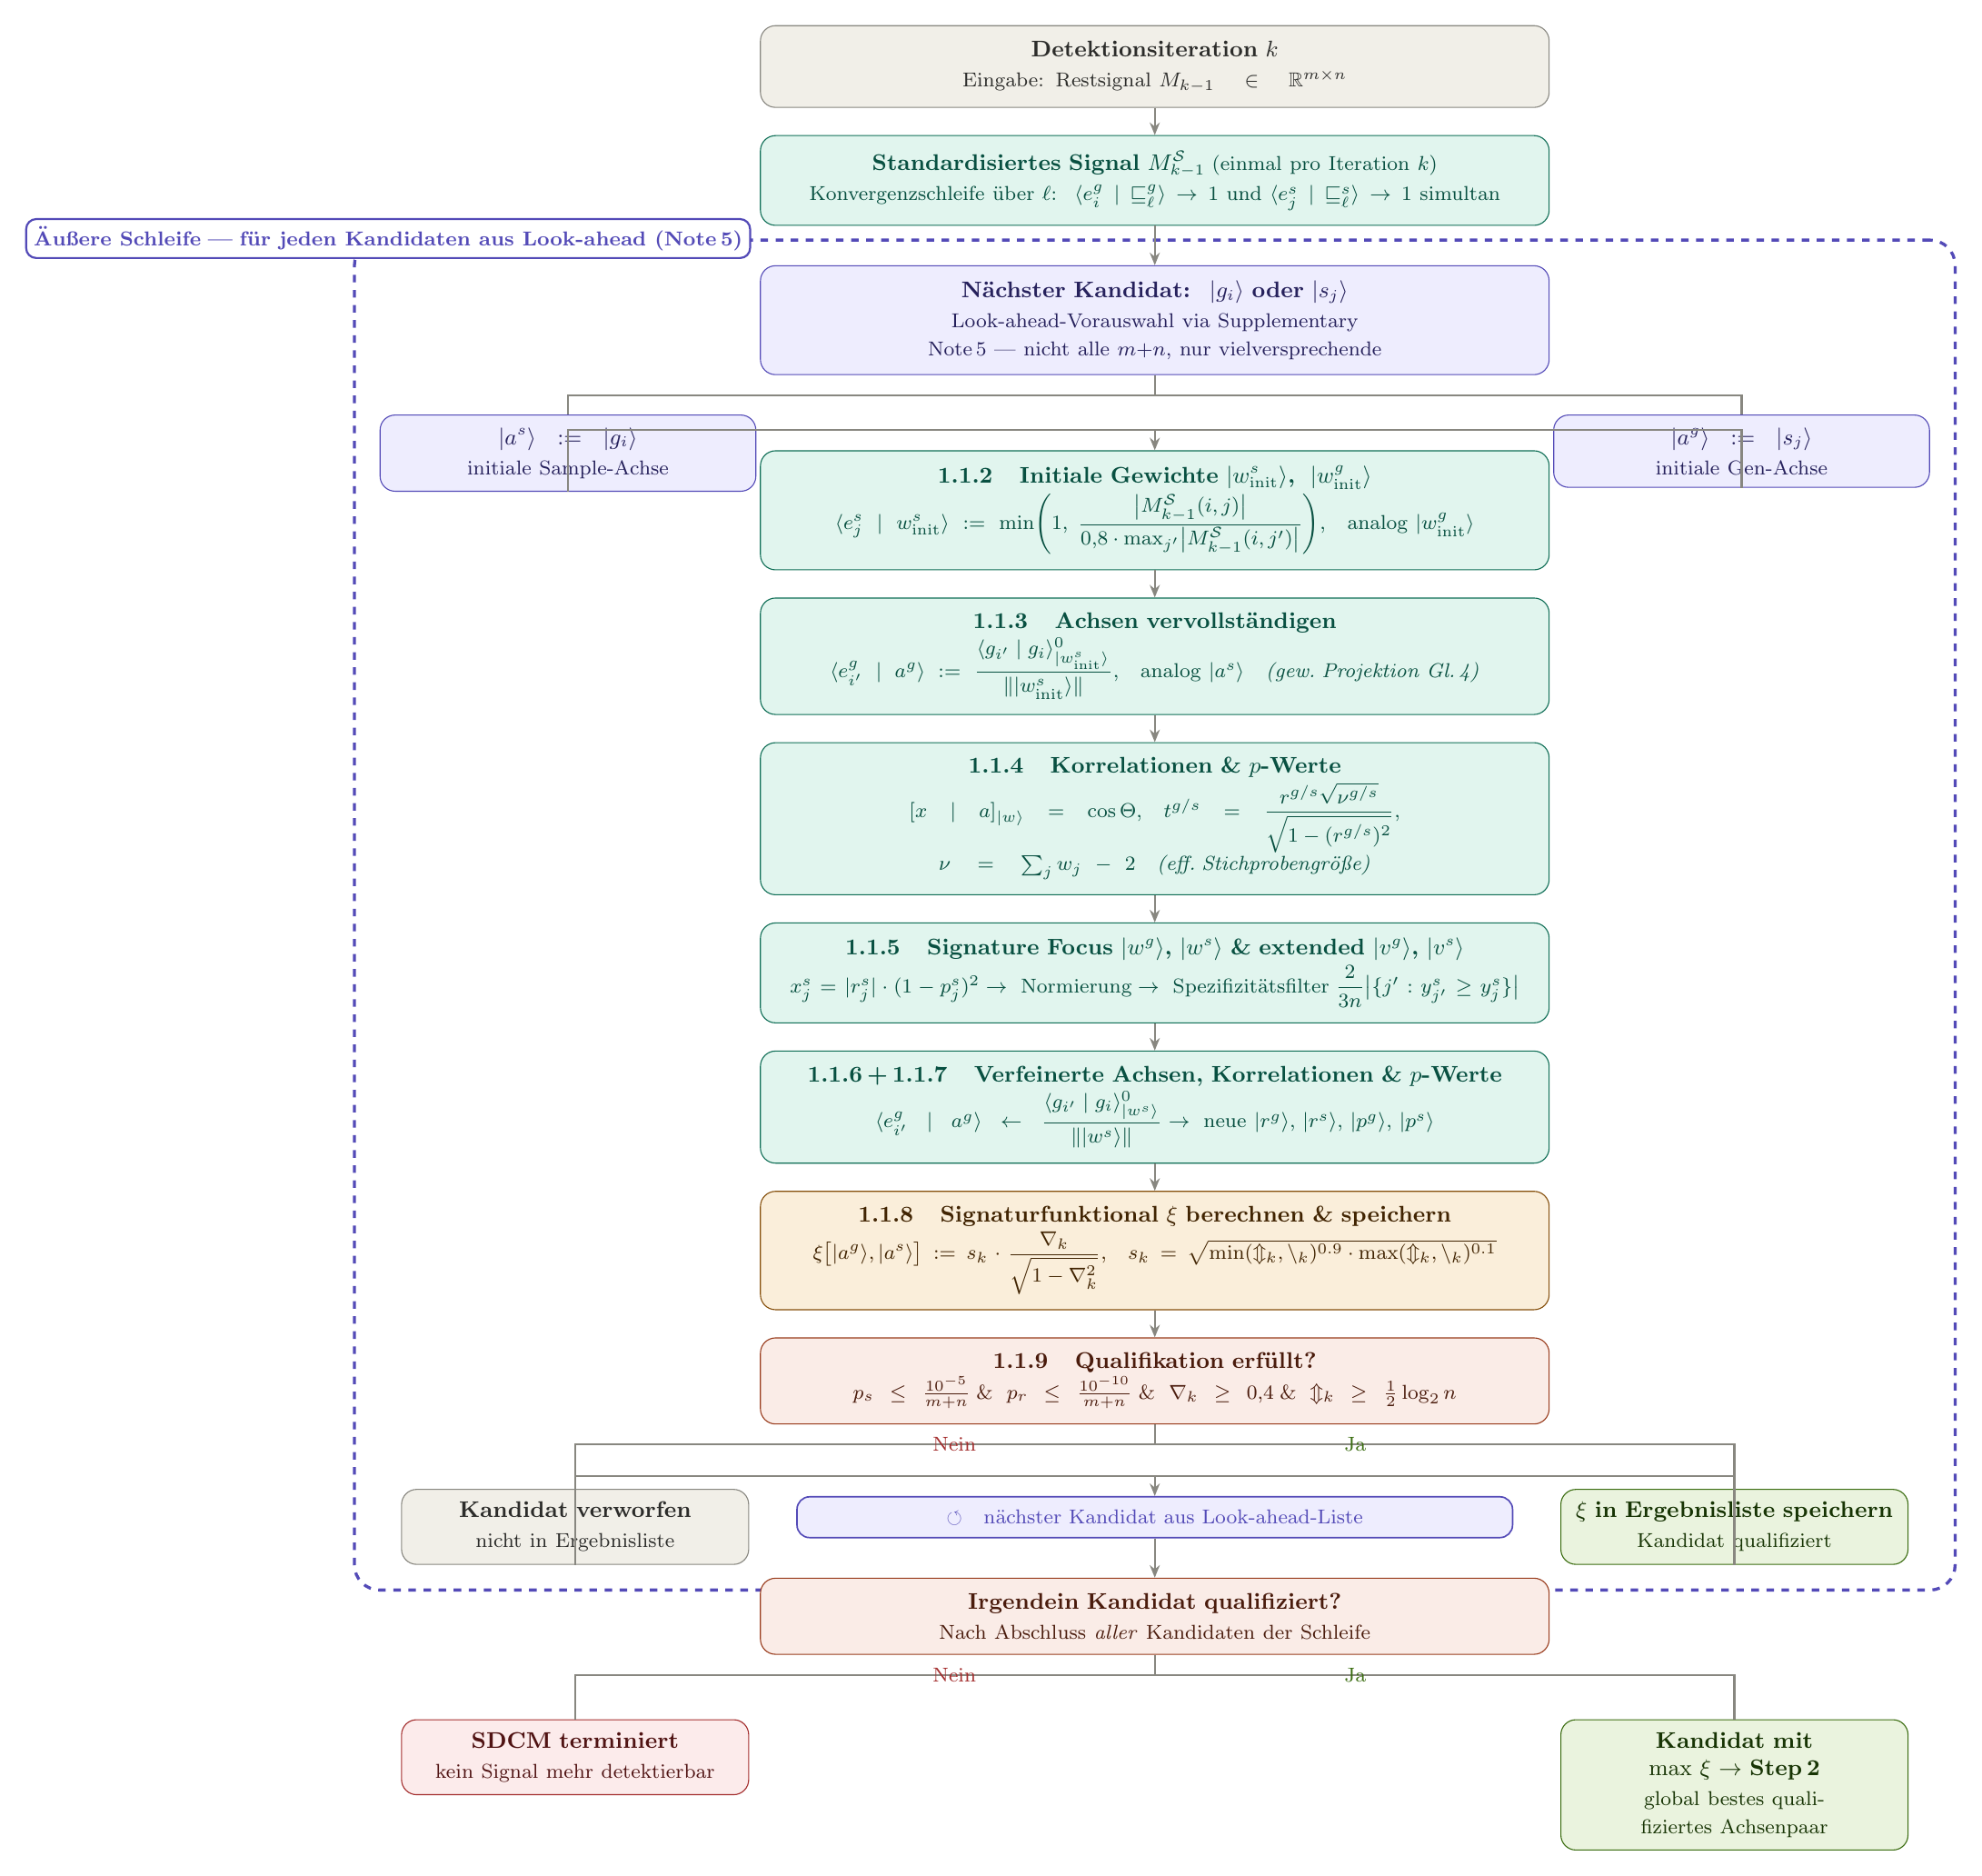
\begin{tikzpicture}[node distance=0.38cm]

% (0) Start
\node[sdcm@gray] (start) {%
  \textbf{Detektionsiteration $k$}\\[1pt]
  {\footnotesize Eingabe: Restsignal $M_{k-1} \in \mathbb{R}^{m \times n}$}%
};

% (1) Standardisierung — once per iteration k, OUTSIDE the loop
\node[sdcm@teal, below=of start] (std) {%
  \textbf{Standardisiertes Signal $M^{\mathcal{S}}_{k-1}$}%
  \;{\footnotesize (einmal pro Iteration $k$)}\\[1pt]
  {\footnotesize Konvergenzschleife über $\ell$:\;
   $\langle e^g_i \mid \mathcal{v}^g_\ell \rangle \to 1$ und
   $\langle e^s_j \mid \mathcal{v}^s_\ell \rangle \to 1$ simultan}%
};

% (2) Candidate — first node inside outer loop
\node[sdcm@purp, below=0.55cm of std] (cand) {%
  \textbf{Nächster Kandidat:\; $|g_i\rangle$ oder $|s_j\rangle$}\\[1pt]
  {\footnotesize Look-ahead-Vorauswahl via Supplementary Note\,5
   — nicht alle $m{+}n$, nur vielversprechende}%
};

% (2a/2b) Branch boxes
\node[sdcm@purpsm, below left=0.55cm and 0.05cm of cand]  (branchL)
  {\textbf{$|a^s\rangle := |g_i\rangle$}\\[1pt]{\footnotesize initiale Sample-Achse}};
\node[sdcm@purpsm, below right=0.55cm and 0.05cm of cand] (branchR)
  {\textbf{$|a^g\rangle := |s_j\rangle$}\\[1pt]{\footnotesize initiale Gen-Achse}};

% (3) Initial weights
\node[sdcm@teal, below=1.05cm of cand] (wini) {%
  \textbf{1.1.2\quad Initiale Gewichte
    $|w^s_\mathrm{init}\rangle$,\; $|w^g_\mathrm{init}\rangle$}\\[1pt]
  {\footnotesize $\displaystyle
    \langle e^s_j \mid w^s_\mathrm{init}\rangle
    := \min\!\left(1,\;
       \frac{\bigl|M^{\mathcal{S}}_{k-1}(i,j)\bigr|}
            {0{,}8\cdot\max_{j'}\bigl|M^{\mathcal{S}}_{k-1}(i,j')\bigr|}
    \right)$,\quad analog $|w^g_\mathrm{init}\rangle$}%
};

% (4) Complete axes
\node[sdcm@teal, below=of wini] (axes) {%
  \textbf{1.1.3\quad Achsen vervollständigen}\\[1pt]
  {\footnotesize $\displaystyle
    \langle e^g_{i'} \mid a^g\rangle
    := \frac{\langle g_{i'} \mid g_i\rangle^0_{|w^s_\mathrm{init}\rangle}}
            {\||w^s_\mathrm{init}\rangle\|}$,\quad
   analog $|a^s\rangle$\quad\textit{(gew.\;Projektion Gl.\,4)}}%
};

% (5) Correlations & p-values
\node[sdcm@teal, below=of axes] (corr) {%
  \textbf{1.1.4\quad Korrelationen \& $p$-Werte}\\[1pt]
  {\footnotesize
   $[x \mid a]_{|w\rangle} = \cos\Theta$,\quad
   $t^{g/s} = \dfrac{r^{g/s}\sqrt{\nu^{g/s}}}{\sqrt{1-(r^{g/s})^2}}$,\quad
   $\nu = \textstyle\sum_j w_j - 2$\quad\textit{(eff.\;Stichprobengröße)}}%
};

% (6) Signature Focus
\node[sdcm@teal, below=of corr] (focus) {%
  \textbf{1.1.5\quad Signature Focus
    $|w^g\rangle$, $|w^s\rangle$ \& extended $|v^g\rangle$, $|v^s\rangle$}\\[1pt]
  {\footnotesize
   $x^s_j = |r^s_j|\cdot(1-p^s_j)^2$\;$\to$\;
   Normierung\;$\to$\;
   Spezifizitätsfilter\;$\dfrac{2}{3n}\bigl|\{j': y^s_{j'}\ge y^s_j\}\bigr|$}%
};

% (7) Refined axes
\node[sdcm@teal, below=of focus] (refit) {%
  \textbf{1.1.6\,+\,1.1.7\quad Verfeinerte Achsen, Korrelationen \& $p$-Werte}\\[1pt]
  {\footnotesize
   $\langle e^g_{i'} \mid a^g\rangle
    \leftarrow \dfrac{\langle g_{i'}\mid g_i\rangle^0_{|w^s\rangle}}
                     {\||w^s\rangle\|}$\;$\to$\;
   neue $|r^g\rangle,\,|r^s\rangle,\,|p^g\rangle,\,|p^s\rangle$}%
};

% (8) Signature functional
\node[sdcm@ambr, below=of refit] (xi) {%
  \textbf{1.1.8\quad Signaturfunktional $\xi$ berechnen \& speichern}\\[1pt]
  {\footnotesize $\displaystyle
    \xi\bigl[|a^g\rangle,|a^s\rangle\bigr]
    := s_k\cdot\frac{\mathcal{r}_k}{\sqrt{1-\mathcal{r}_k^2}}$,\quad
   $s_k=\sqrt{\min(\mathcal{m}_k,\mathcal{n}_k)^{0.9}
               \cdot\max(\mathcal{m}_k,\mathcal{n}_k)^{0.1}}$}%
};

% (9) Qualification
\node[sdcm@corl, below=of xi] (qual) {%
  \textbf{1.1.9\quad Qualifikation erfüllt?}\\[1pt]
  {\footnotesize
   $p_s\le\tfrac{10^{-5}}{m+n}$\;\&\;
   $p_r\le\tfrac{10^{-10}}{m+n}$\;\&\;
   $\mathcal{r}_k\ge0{,}4$\;\&\;
   $\mathcal{m}_k\ge\tfrac{1}{2}\log_2 n$}%
};

% Qualification branch outcomes
\node[sdcm@disc, below left=0.9cm  and 0.15cm of qual] (disc)
  {\textbf{Kandidat verworfen}\\[1pt]{\footnotesize nicht in Ergebnisliste}};
\node[sdcm@gren, below right=0.9cm and 0.15cm of qual] (save)
  {\textbf{$\xi$ in Ergebnisliste speichern}\\[1pt]{\footnotesize Kandidat qualifiziert}};

% Loop-back banner
\node[sdcm@loop, below=1.0cm of qual] (loopback)
  {$\circlearrowleft$\quad nächster Kandidat aus Look-ahead-Liste};

% Final decision (outside loop)
\node[sdcm@corl, below=0.55cm of loopback] (anyq) {%
  \textbf{Irgendein Kandidat qualifiziert?}\\[1pt]
  {\footnotesize Nach Abschluss \emph{aller} Kandidaten der Schleife}%
};

% Final outcomes
\node[sdcm@red,  below left=0.9cm  and 0.15cm of anyq] (term)
  {\textbf{SDCM terminiert}\\[1pt]{\footnotesize kein Signal mehr detektierbar}};
\node[sdcm@gren, below right=0.9cm and 0.15cm of anyq] (step2)
  {\textbf{Kandidat mit $\max\,\xi$ $\to$ Step\,2}\\[1pt]
   {\footnotesize global bestes qualifiziertes Achsenpaar}};

% Outer loop dashed frame
\begin{scope}[on background layer]
  \node[draw=sdcm@purp@bd, line width=1.2pt, dashed, fill=none,
    rounded corners=10pt, inner sep=10pt,
    fit=(cand)(branchL)(branchR)(wini)(axes)(corr)
        (focus)(refit)(xi)(qual)(disc)(save)(loopback)
  ] (outerloop) {};
\end{scope}
\node[fill=white, draw=sdcm@purp@bd, line width=0.8pt, rounded corners=4pt,
  inner sep=3pt, font=\footnotesize\bfseries, text=sdcm@purp@bd
] at (outerloop.north west) [xshift=14pt]
  {Äußere Schleife\;—\;für jeden Kandidaten aus Look-ahead (Note\,5)};

% Arrows
\draw[sdcm@arr]  (start.south) -- (std.north);
\draw[sdcm@arr]  (std.south)   -- (cand.north);

\coordinate (splitPt) at ($(cand.south)+(0,-0.28)$);
\draw[sdcm@line] (cand.south) -- (splitPt);
\draw[sdcm@line] (splitPt) -| (branchL.north);
\draw[sdcm@line] (splitPt) -| (branchR.north);

\coordinate (mergePt) at ($(wini.north)+(0,0.28)$);
\draw[sdcm@line] (branchL.south) |- (mergePt);
\draw[sdcm@line] (branchR.south) |- (mergePt);
\draw[sdcm@arr]  (mergePt) -- (wini.north);

\draw[sdcm@arr] (wini.south)  -- (axes.north);
\draw[sdcm@arr] (axes.south)  -- (corr.north);
\draw[sdcm@arr] (corr.south)  -- (focus.north);
\draw[sdcm@arr] (focus.south) -- (refit.north);
\draw[sdcm@arr] (refit.south) -- (xi.north);
\draw[sdcm@arr] (xi.south)    -- (qual.north);

\coordinate (qSplit) at ($(qual.south)+(0,-0.28)$);
\draw[sdcm@line] (qual.south) -- (qSplit);
\draw[sdcm@line] (qSplit) -| (disc.north);
\draw[sdcm@line] (qSplit) -| (save.north);
\node[font=\footnotesize, text=sdcm@red@bd]  at ($(qSplit)+(-2.8,0)$) {Nein};
\node[font=\footnotesize, text=sdcm@gren@bd] at ($(qSplit)+(+2.8,0)$) {Ja};

\coordinate (lbMerge) at ($(loopback.north)+(0,0.28)$);
\draw[sdcm@line] (disc.south) |- (lbMerge);
\draw[sdcm@line] (save.south) |- (lbMerge);
\draw[sdcm@arr]  (lbMerge)   -- (loopback.north);
\draw[sdcm@arr]  (loopback.south) -- (anyq.north);

\coordinate (aSplit) at ($(anyq.south)+(0,-0.28)$);
\draw[sdcm@line] (anyq.south) -- (aSplit);
\draw[sdcm@line] (aSplit) -| (term.north);
\draw[sdcm@line] (aSplit) -| (step2.north);
\node[font=\footnotesize, text=sdcm@red@bd]  at ($(aSplit)+(-2.8,0)$) {Nein};
\node[font=\footnotesize, text=sdcm@gren@bd] at ($(aSplit)+(+2.8,0)$) {Ja};

\end{tikzpicture}
\end{document}}
%%     \caption{SDCM Step 1 -- Search Strategy}
%%   \end{figure}
%%
%% ZERO custom \newcommand definitions — safe with any package combination
%% (physics, braket, etc.).  All names are prefixed sdcm@ to avoid clashes.

\documentclass[tikz, border=10pt]{standalone}
\usepackage{tikz}
\usepackage{amsmath, amssymb}
\usetikzlibrary{shapes.geometric, arrows.meta, positioning, fit, backgrounds, calc}

% Colors (hex taken 1:1 from the widget)
\definecolor{sdcm@gray@bg}{RGB}{241,239,232}
\definecolor{sdcm@gray@bd}{RGB}{136,135,128}
\definecolor{sdcm@gray@tx}{RGB}{ 44, 44, 42}
\definecolor{sdcm@teal@bg}{RGB}{225,245,238}
\definecolor{sdcm@teal@bd}{RGB}{ 15,110, 86}
\definecolor{sdcm@teal@tx}{RGB}{  8, 80, 65}
\definecolor{sdcm@purp@bg}{RGB}{238,237,254}
\definecolor{sdcm@purp@bd}{RGB}{ 83, 74,183}
\definecolor{sdcm@purp@tx}{RGB}{ 38, 33, 92}
\definecolor{sdcm@ambr@bg}{RGB}{250,238,218}
\definecolor{sdcm@ambr@bd}{RGB}{133, 79, 11}
\definecolor{sdcm@ambr@tx}{RGB}{ 65, 36,  2}
\definecolor{sdcm@corl@bg}{RGB}{250,236,231}
\definecolor{sdcm@corl@bd}{RGB}{153, 60, 29}
\definecolor{sdcm@corl@tx}{RGB}{ 74, 27, 12}
\definecolor{sdcm@gren@bg}{RGB}{234,243,222}
\definecolor{sdcm@gren@bd}{RGB}{ 59,109, 17}
\definecolor{sdcm@gren@tx}{RGB}{ 23, 52,  4}
\definecolor{sdcm@red@bg} {RGB}{252,235,235}
\definecolor{sdcm@red@bd} {RGB}{163, 45, 45}
\definecolor{sdcm@red@tx} {RGB}{ 80, 19, 19}

% TikZ styles (all prefixed sdcm@ to avoid name clashes)
\tikzset{
  sdcm@base/.style={rectangle, rounded corners=6pt,
    minimum width=11cm, minimum height=0.9cm, text width=10.6cm,
    align=center, font=\small, inner sep=6pt, line width=0.4pt},
  sdcm@gray/.style={sdcm@base,
    fill=sdcm@gray@bg, draw=sdcm@gray@bd, text=sdcm@gray@tx},
  sdcm@teal/.style={sdcm@base,
    fill=sdcm@teal@bg, draw=sdcm@teal@bd, text=sdcm@teal@tx},
  sdcm@purp/.style={sdcm@base,
    fill=sdcm@purp@bg, draw=sdcm@purp@bd, text=sdcm@purp@tx},
  sdcm@ambr/.style={sdcm@base,
    fill=sdcm@ambr@bg, draw=sdcm@ambr@bd, text=sdcm@ambr@tx},
  sdcm@corl/.style={sdcm@base,
    fill=sdcm@corl@bg, draw=sdcm@corl@bd, text=sdcm@corl@tx},
  sdcm@purpsm/.style={rectangle, rounded corners=6pt,
    minimum width=5.2cm, minimum height=0.85cm, text width=4.9cm,
    align=center, font=\small, inner sep=5pt, line width=0.4pt,
    fill=sdcm@purp@bg, draw=sdcm@purp@bd, text=sdcm@purp@tx},
  sdcm@gren/.style={rectangle, rounded corners=6pt,
    minimum width=4.8cm, minimum height=0.85cm, text width=4.5cm,
    align=center, font=\small, inner sep=5pt, line width=0.4pt,
    fill=sdcm@gren@bg, draw=sdcm@gren@bd, text=sdcm@gren@tx},
  sdcm@red/.style={rectangle, rounded corners=6pt,
    minimum width=4.8cm, minimum height=0.85cm, text width=4.5cm,
    align=center, font=\small, inner sep=5pt, line width=0.4pt,
    fill=sdcm@red@bg, draw=sdcm@red@bd, text=sdcm@red@tx},
  sdcm@disc/.style={rectangle, rounded corners=6pt,
    minimum width=4.8cm, minimum height=0.85cm, text width=4.5cm,
    align=center, font=\small, inner sep=5pt, line width=0.4pt,
    fill=sdcm@gray@bg, draw=sdcm@gray@bd, text=sdcm@gray@tx},
  sdcm@loop/.style={rectangle, rounded corners=5pt,
    fill=sdcm@purp@bg, draw=sdcm@purp@bd,
    font=\footnotesize, text=sdcm@purp@bd,
    inner sep=5pt, line width=0.6pt,
    minimum width=10cm, text width=9.6cm, align=center},
  sdcm@arr/.style={-{Stealth[length=5pt,width=4pt]},
    line width=0.8pt, color=sdcm@gray@bd},
  sdcm@line/.style={line width=0.8pt, color=sdcm@gray@bd},
}

\begin{document}
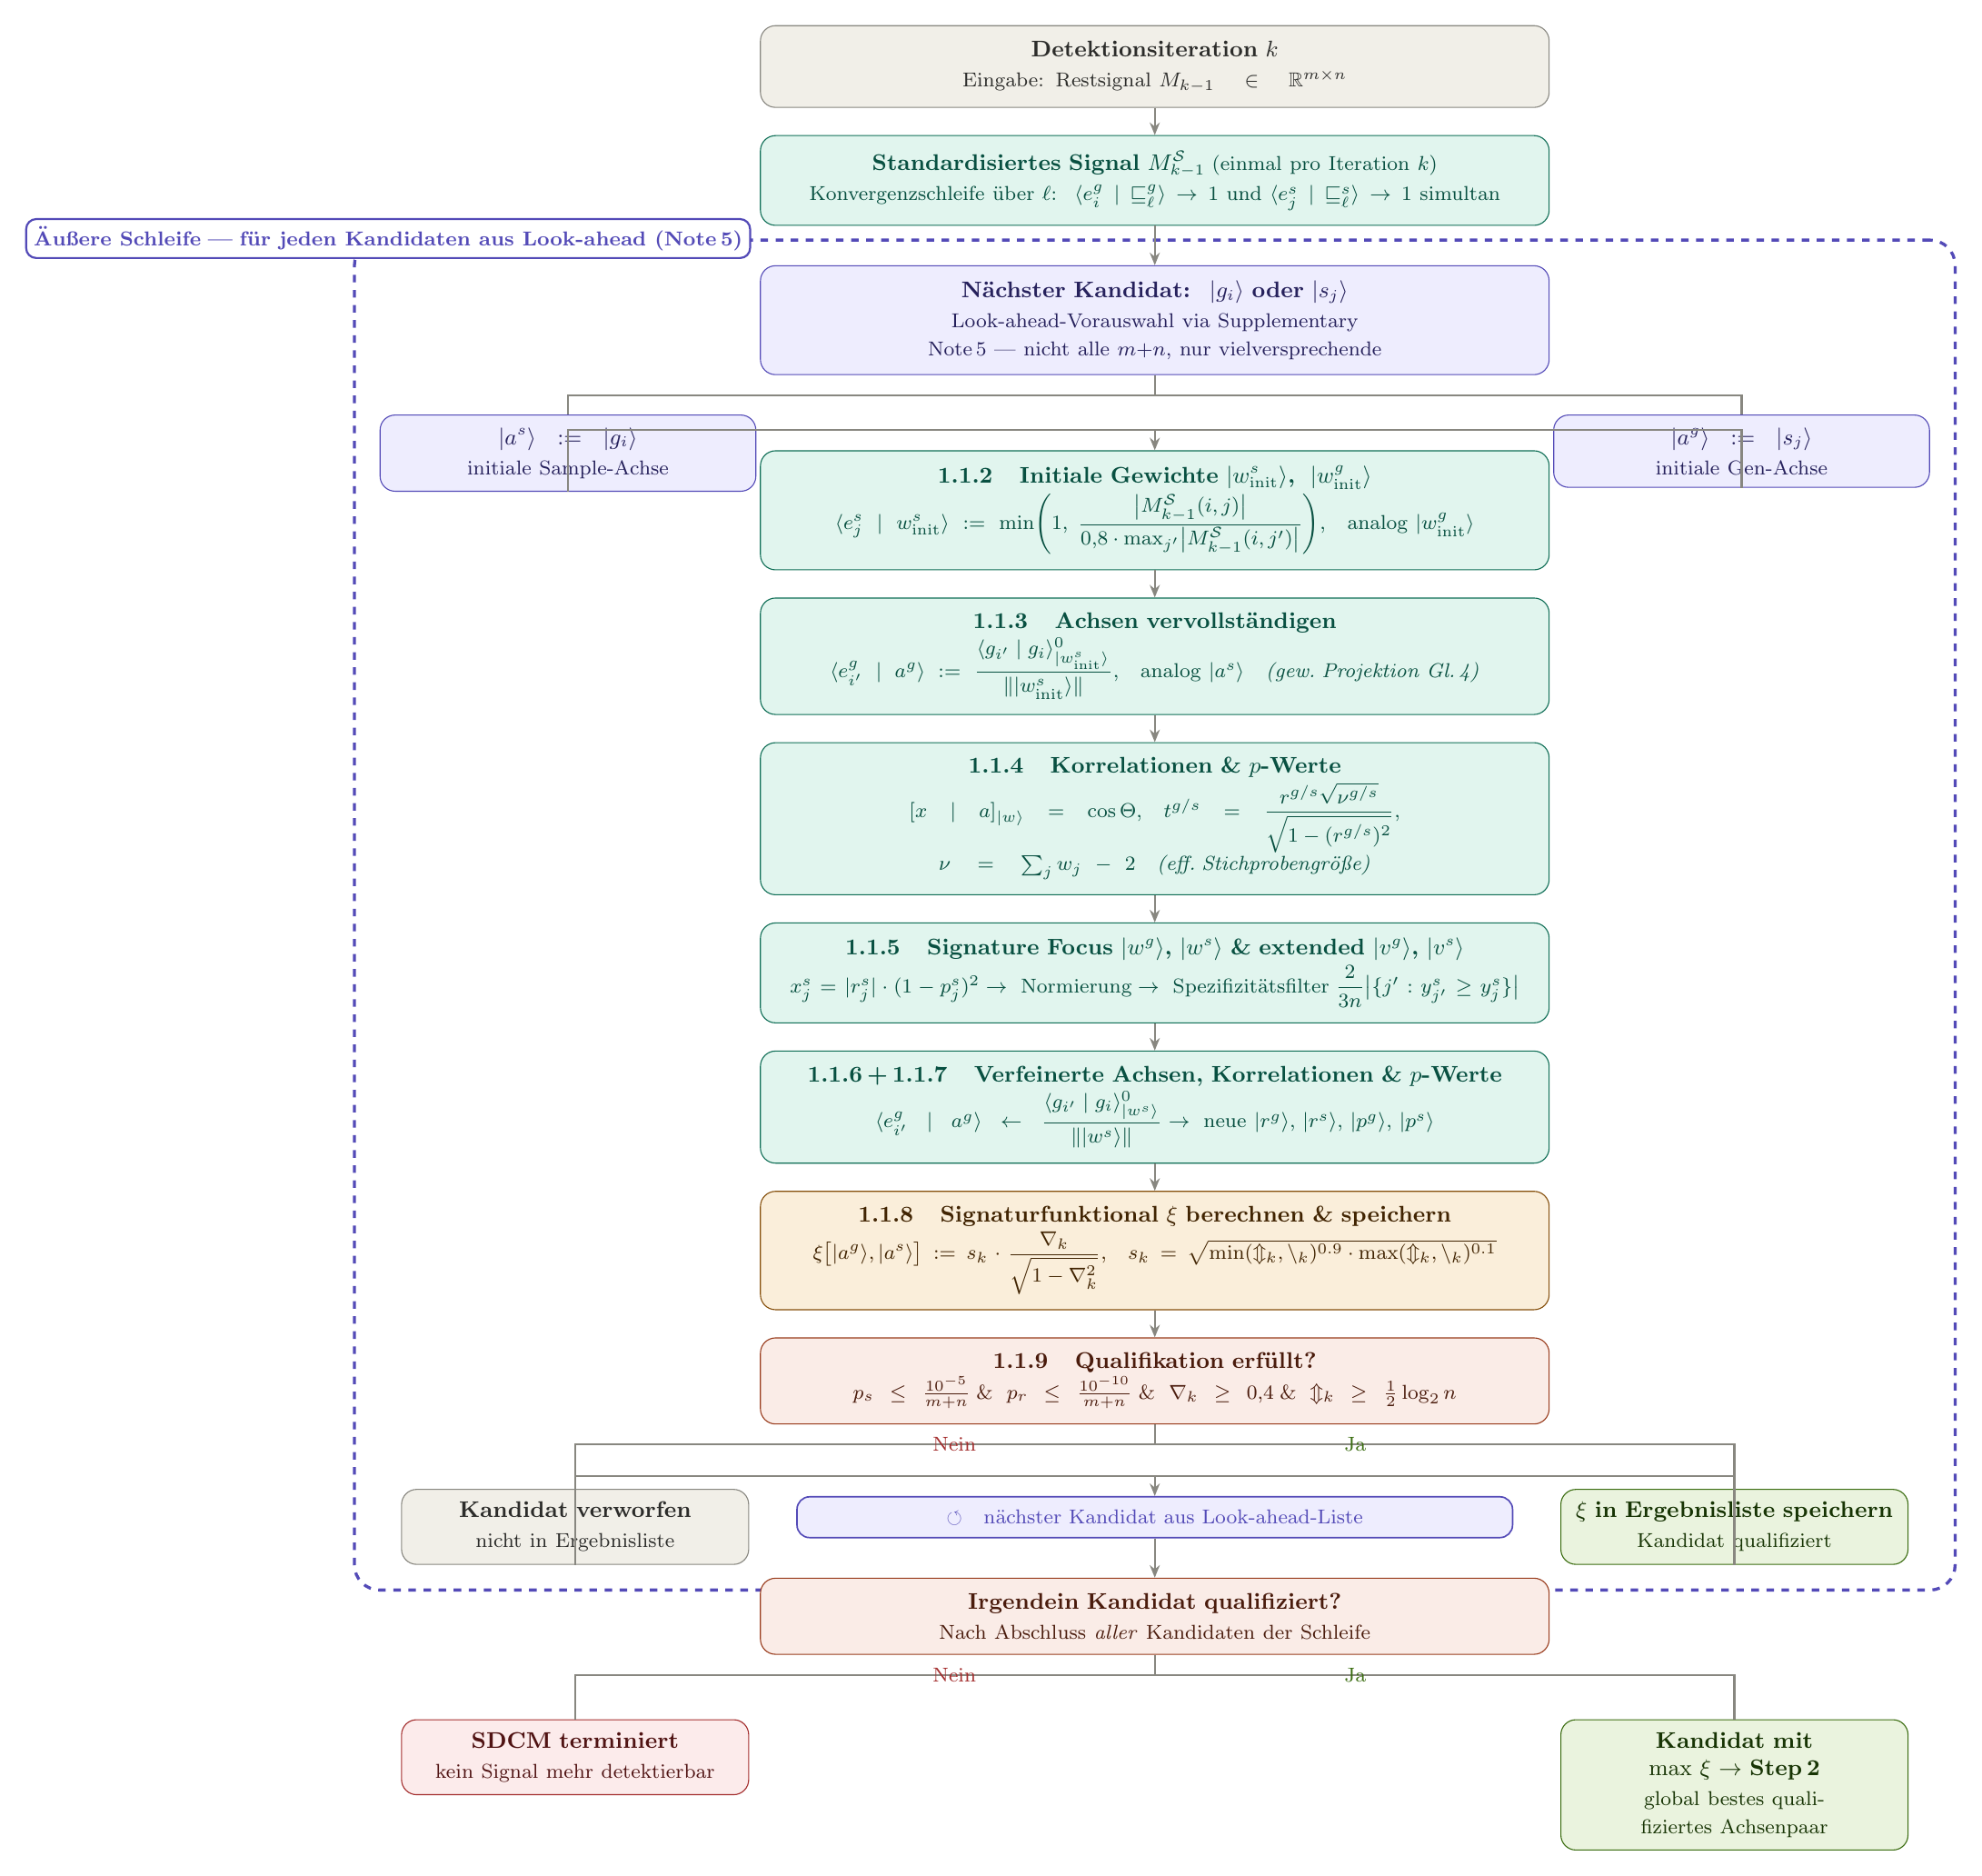
\begin{tikzpicture}[node distance=0.38cm]

% (0) Start
\node[sdcm@gray] (start) {%
  \textbf{Detektionsiteration $k$}\\[1pt]
  {\footnotesize Eingabe: Restsignal $M_{k-1} \in \mathbb{R}^{m \times n}$}%
};

% (1) Standardisierung — once per iteration k, OUTSIDE the loop
\node[sdcm@teal, below=of start] (std) {%
  \textbf{Standardisiertes Signal $M^{\mathcal{S}}_{k-1}$}%
  \;{\footnotesize (einmal pro Iteration $k$)}\\[1pt]
  {\footnotesize Konvergenzschleife über $\ell$:\;
   $\langle e^g_i \mid \mathcal{v}^g_\ell \rangle \to 1$ und
   $\langle e^s_j \mid \mathcal{v}^s_\ell \rangle \to 1$ simultan}%
};

% (2) Candidate — first node inside outer loop
\node[sdcm@purp, below=0.55cm of std] (cand) {%
  \textbf{Nächster Kandidat:\; $|g_i\rangle$ oder $|s_j\rangle$}\\[1pt]
  {\footnotesize Look-ahead-Vorauswahl via Supplementary Note\,5
   — nicht alle $m{+}n$, nur vielversprechende}%
};

% (2a/2b) Branch boxes
\node[sdcm@purpsm, below left=0.55cm and 0.05cm of cand]  (branchL)
  {\textbf{$|a^s\rangle := |g_i\rangle$}\\[1pt]{\footnotesize initiale Sample-Achse}};
\node[sdcm@purpsm, below right=0.55cm and 0.05cm of cand] (branchR)
  {\textbf{$|a^g\rangle := |s_j\rangle$}\\[1pt]{\footnotesize initiale Gen-Achse}};

% (3) Initial weights
\node[sdcm@teal, below=1.05cm of cand] (wini) {%
  \textbf{1.1.2\quad Initiale Gewichte
    $|w^s_\mathrm{init}\rangle$,\; $|w^g_\mathrm{init}\rangle$}\\[1pt]
  {\footnotesize $\displaystyle
    \langle e^s_j \mid w^s_\mathrm{init}\rangle
    := \min\!\left(1,\;
       \frac{\bigl|M^{\mathcal{S}}_{k-1}(i,j)\bigr|}
            {0{,}8\cdot\max_{j'}\bigl|M^{\mathcal{S}}_{k-1}(i,j')\bigr|}
    \right)$,\quad analog $|w^g_\mathrm{init}\rangle$}%
};

% (4) Complete axes
\node[sdcm@teal, below=of wini] (axes) {%
  \textbf{1.1.3\quad Achsen vervollständigen}\\[1pt]
  {\footnotesize $\displaystyle
    \langle e^g_{i'} \mid a^g\rangle
    := \frac{\langle g_{i'} \mid g_i\rangle^0_{|w^s_\mathrm{init}\rangle}}
            {\||w^s_\mathrm{init}\rangle\|}$,\quad
   analog $|a^s\rangle$\quad\textit{(gew.\;Projektion Gl.\,4)}}%
};

% (5) Correlations & p-values
\node[sdcm@teal, below=of axes] (corr) {%
  \textbf{1.1.4\quad Korrelationen \& $p$-Werte}\\[1pt]
  {\footnotesize
   $[x \mid a]_{|w\rangle} = \cos\Theta$,\quad
   $t^{g/s} = \dfrac{r^{g/s}\sqrt{\nu^{g/s}}}{\sqrt{1-(r^{g/s})^2}}$,\quad
   $\nu = \textstyle\sum_j w_j - 2$\quad\textit{(eff.\;Stichprobengröße)}}%
};

% (6) Signature Focus
\node[sdcm@teal, below=of corr] (focus) {%
  \textbf{1.1.5\quad Signature Focus
    $|w^g\rangle$, $|w^s\rangle$ \& extended $|v^g\rangle$, $|v^s\rangle$}\\[1pt]
  {\footnotesize
   $x^s_j = |r^s_j|\cdot(1-p^s_j)^2$\;$\to$\;
   Normierung\;$\to$\;
   Spezifizitätsfilter\;$\dfrac{2}{3n}\bigl|\{j': y^s_{j'}\ge y^s_j\}\bigr|$}%
};

% (7) Refined axes
\node[sdcm@teal, below=of focus] (refit) {%
  \textbf{1.1.6\,+\,1.1.7\quad Verfeinerte Achsen, Korrelationen \& $p$-Werte}\\[1pt]
  {\footnotesize
   $\langle e^g_{i'} \mid a^g\rangle
    \leftarrow \dfrac{\langle g_{i'}\mid g_i\rangle^0_{|w^s\rangle}}
                     {\||w^s\rangle\|}$\;$\to$\;
   neue $|r^g\rangle,\,|r^s\rangle,\,|p^g\rangle,\,|p^s\rangle$}%
};

% (8) Signature functional
\node[sdcm@ambr, below=of refit] (xi) {%
  \textbf{1.1.8\quad Signaturfunktional $\xi$ berechnen \& speichern}\\[1pt]
  {\footnotesize $\displaystyle
    \xi\bigl[|a^g\rangle,|a^s\rangle\bigr]
    := s_k\cdot\frac{\mathcal{r}_k}{\sqrt{1-\mathcal{r}_k^2}}$,\quad
   $s_k=\sqrt{\min(\mathcal{m}_k,\mathcal{n}_k)^{0.9}
               \cdot\max(\mathcal{m}_k,\mathcal{n}_k)^{0.1}}$}%
};

% (9) Qualification
\node[sdcm@corl, below=of xi] (qual) {%
  \textbf{1.1.9\quad Qualifikation erfüllt?}\\[1pt]
  {\footnotesize
   $p_s\le\tfrac{10^{-5}}{m+n}$\;\&\;
   $p_r\le\tfrac{10^{-10}}{m+n}$\;\&\;
   $\mathcal{r}_k\ge0{,}4$\;\&\;
   $\mathcal{m}_k\ge\tfrac{1}{2}\log_2 n$}%
};

% Qualification branch outcomes
\node[sdcm@disc, below left=0.9cm  and 0.15cm of qual] (disc)
  {\textbf{Kandidat verworfen}\\[1pt]{\footnotesize nicht in Ergebnisliste}};
\node[sdcm@gren, below right=0.9cm and 0.15cm of qual] (save)
  {\textbf{$\xi$ in Ergebnisliste speichern}\\[1pt]{\footnotesize Kandidat qualifiziert}};

% Loop-back banner
\node[sdcm@loop, below=1.0cm of qual] (loopback)
  {$\circlearrowleft$\quad nächster Kandidat aus Look-ahead-Liste};

% Final decision (outside loop)
\node[sdcm@corl, below=0.55cm of loopback] (anyq) {%
  \textbf{Irgendein Kandidat qualifiziert?}\\[1pt]
  {\footnotesize Nach Abschluss \emph{aller} Kandidaten der Schleife}%
};

% Final outcomes
\node[sdcm@red,  below left=0.9cm  and 0.15cm of anyq] (term)
  {\textbf{SDCM terminiert}\\[1pt]{\footnotesize kein Signal mehr detektierbar}};
\node[sdcm@gren, below right=0.9cm and 0.15cm of anyq] (step2)
  {\textbf{Kandidat mit $\max\,\xi$ $\to$ Step\,2}\\[1pt]
   {\footnotesize global bestes qualifiziertes Achsenpaar}};

% Outer loop dashed frame
\begin{scope}[on background layer]
  \node[draw=sdcm@purp@bd, line width=1.2pt, dashed, fill=none,
    rounded corners=10pt, inner sep=10pt,
    fit=(cand)(branchL)(branchR)(wini)(axes)(corr)
        (focus)(refit)(xi)(qual)(disc)(save)(loopback)
  ] (outerloop) {};
\end{scope}
\node[fill=white, draw=sdcm@purp@bd, line width=0.8pt, rounded corners=4pt,
  inner sep=3pt, font=\footnotesize\bfseries, text=sdcm@purp@bd
] at (outerloop.north west) [xshift=14pt]
  {Äußere Schleife\;—\;für jeden Kandidaten aus Look-ahead (Note\,5)};

% Arrows
\draw[sdcm@arr]  (start.south) -- (std.north);
\draw[sdcm@arr]  (std.south)   -- (cand.north);

\coordinate (splitPt) at ($(cand.south)+(0,-0.28)$);
\draw[sdcm@line] (cand.south) -- (splitPt);
\draw[sdcm@line] (splitPt) -| (branchL.north);
\draw[sdcm@line] (splitPt) -| (branchR.north);

\coordinate (mergePt) at ($(wini.north)+(0,0.28)$);
\draw[sdcm@line] (branchL.south) |- (mergePt);
\draw[sdcm@line] (branchR.south) |- (mergePt);
\draw[sdcm@arr]  (mergePt) -- (wini.north);

\draw[sdcm@arr] (wini.south)  -- (axes.north);
\draw[sdcm@arr] (axes.south)  -- (corr.north);
\draw[sdcm@arr] (corr.south)  -- (focus.north);
\draw[sdcm@arr] (focus.south) -- (refit.north);
\draw[sdcm@arr] (refit.south) -- (xi.north);
\draw[sdcm@arr] (xi.south)    -- (qual.north);

\coordinate (qSplit) at ($(qual.south)+(0,-0.28)$);
\draw[sdcm@line] (qual.south) -- (qSplit);
\draw[sdcm@line] (qSplit) -| (disc.north);
\draw[sdcm@line] (qSplit) -| (save.north);
\node[font=\footnotesize, text=sdcm@red@bd]  at ($(qSplit)+(-2.8,0)$) {Nein};
\node[font=\footnotesize, text=sdcm@gren@bd] at ($(qSplit)+(+2.8,0)$) {Ja};

\coordinate (lbMerge) at ($(loopback.north)+(0,0.28)$);
\draw[sdcm@line] (disc.south) |- (lbMerge);
\draw[sdcm@line] (save.south) |- (lbMerge);
\draw[sdcm@arr]  (lbMerge)   -- (loopback.north);
\draw[sdcm@arr]  (loopback.south) -- (anyq.north);

\coordinate (aSplit) at ($(anyq.south)+(0,-0.28)$);
\draw[sdcm@line] (anyq.south) -- (aSplit);
\draw[sdcm@line] (aSplit) -| (term.north);
\draw[sdcm@line] (aSplit) -| (step2.north);
\node[font=\footnotesize, text=sdcm@red@bd]  at ($(aSplit)+(-2.8,0)$) {Nein};
\node[font=\footnotesize, text=sdcm@gren@bd] at ($(aSplit)+(+2.8,0)$) {Ja};

\end{tikzpicture}
\end{document}}
%%     \caption{SDCM Step 1 -- Search Strategy}
%%   \end{figure}
%%
%% ZERO custom \newcommand definitions — safe with any package combination
%% (physics, braket, etc.).  All names are prefixed sdcm@ to avoid clashes.

\documentclass[tikz, border=10pt]{standalone}
\usepackage{tikz}
\usepackage{amsmath, amssymb}
\usetikzlibrary{shapes.geometric, arrows.meta, positioning, fit, backgrounds, calc}

% Colors (hex taken 1:1 from the widget)
\definecolor{sdcm@gray@bg}{RGB}{241,239,232}
\definecolor{sdcm@gray@bd}{RGB}{136,135,128}
\definecolor{sdcm@gray@tx}{RGB}{ 44, 44, 42}
\definecolor{sdcm@teal@bg}{RGB}{225,245,238}
\definecolor{sdcm@teal@bd}{RGB}{ 15,110, 86}
\definecolor{sdcm@teal@tx}{RGB}{  8, 80, 65}
\definecolor{sdcm@purp@bg}{RGB}{238,237,254}
\definecolor{sdcm@purp@bd}{RGB}{ 83, 74,183}
\definecolor{sdcm@purp@tx}{RGB}{ 38, 33, 92}
\definecolor{sdcm@ambr@bg}{RGB}{250,238,218}
\definecolor{sdcm@ambr@bd}{RGB}{133, 79, 11}
\definecolor{sdcm@ambr@tx}{RGB}{ 65, 36,  2}
\definecolor{sdcm@corl@bg}{RGB}{250,236,231}
\definecolor{sdcm@corl@bd}{RGB}{153, 60, 29}
\definecolor{sdcm@corl@tx}{RGB}{ 74, 27, 12}
\definecolor{sdcm@gren@bg}{RGB}{234,243,222}
\definecolor{sdcm@gren@bd}{RGB}{ 59,109, 17}
\definecolor{sdcm@gren@tx}{RGB}{ 23, 52,  4}
\definecolor{sdcm@red@bg} {RGB}{252,235,235}
\definecolor{sdcm@red@bd} {RGB}{163, 45, 45}
\definecolor{sdcm@red@tx} {RGB}{ 80, 19, 19}

% TikZ styles (all prefixed sdcm@ to avoid name clashes)
\tikzset{
  sdcm@base/.style={rectangle, rounded corners=6pt,
    minimum width=11cm, minimum height=0.9cm, text width=10.6cm,
    align=center, font=\small, inner sep=6pt, line width=0.4pt},
  sdcm@gray/.style={sdcm@base,
    fill=sdcm@gray@bg, draw=sdcm@gray@bd, text=sdcm@gray@tx},
  sdcm@teal/.style={sdcm@base,
    fill=sdcm@teal@bg, draw=sdcm@teal@bd, text=sdcm@teal@tx},
  sdcm@purp/.style={sdcm@base,
    fill=sdcm@purp@bg, draw=sdcm@purp@bd, text=sdcm@purp@tx},
  sdcm@ambr/.style={sdcm@base,
    fill=sdcm@ambr@bg, draw=sdcm@ambr@bd, text=sdcm@ambr@tx},
  sdcm@corl/.style={sdcm@base,
    fill=sdcm@corl@bg, draw=sdcm@corl@bd, text=sdcm@corl@tx},
  sdcm@purpsm/.style={rectangle, rounded corners=6pt,
    minimum width=5.2cm, minimum height=0.85cm, text width=4.9cm,
    align=center, font=\small, inner sep=5pt, line width=0.4pt,
    fill=sdcm@purp@bg, draw=sdcm@purp@bd, text=sdcm@purp@tx},
  sdcm@gren/.style={rectangle, rounded corners=6pt,
    minimum width=4.8cm, minimum height=0.85cm, text width=4.5cm,
    align=center, font=\small, inner sep=5pt, line width=0.4pt,
    fill=sdcm@gren@bg, draw=sdcm@gren@bd, text=sdcm@gren@tx},
  sdcm@red/.style={rectangle, rounded corners=6pt,
    minimum width=4.8cm, minimum height=0.85cm, text width=4.5cm,
    align=center, font=\small, inner sep=5pt, line width=0.4pt,
    fill=sdcm@red@bg, draw=sdcm@red@bd, text=sdcm@red@tx},
  sdcm@disc/.style={rectangle, rounded corners=6pt,
    minimum width=4.8cm, minimum height=0.85cm, text width=4.5cm,
    align=center, font=\small, inner sep=5pt, line width=0.4pt,
    fill=sdcm@gray@bg, draw=sdcm@gray@bd, text=sdcm@gray@tx},
  sdcm@loop/.style={rectangle, rounded corners=5pt,
    fill=sdcm@purp@bg, draw=sdcm@purp@bd,
    font=\footnotesize, text=sdcm@purp@bd,
    inner sep=5pt, line width=0.6pt,
    minimum width=10cm, text width=9.6cm, align=center},
  sdcm@arr/.style={-{Stealth[length=5pt,width=4pt]},
    line width=0.8pt, color=sdcm@gray@bd},
  sdcm@line/.style={line width=0.8pt, color=sdcm@gray@bd},
}

\begin{document}
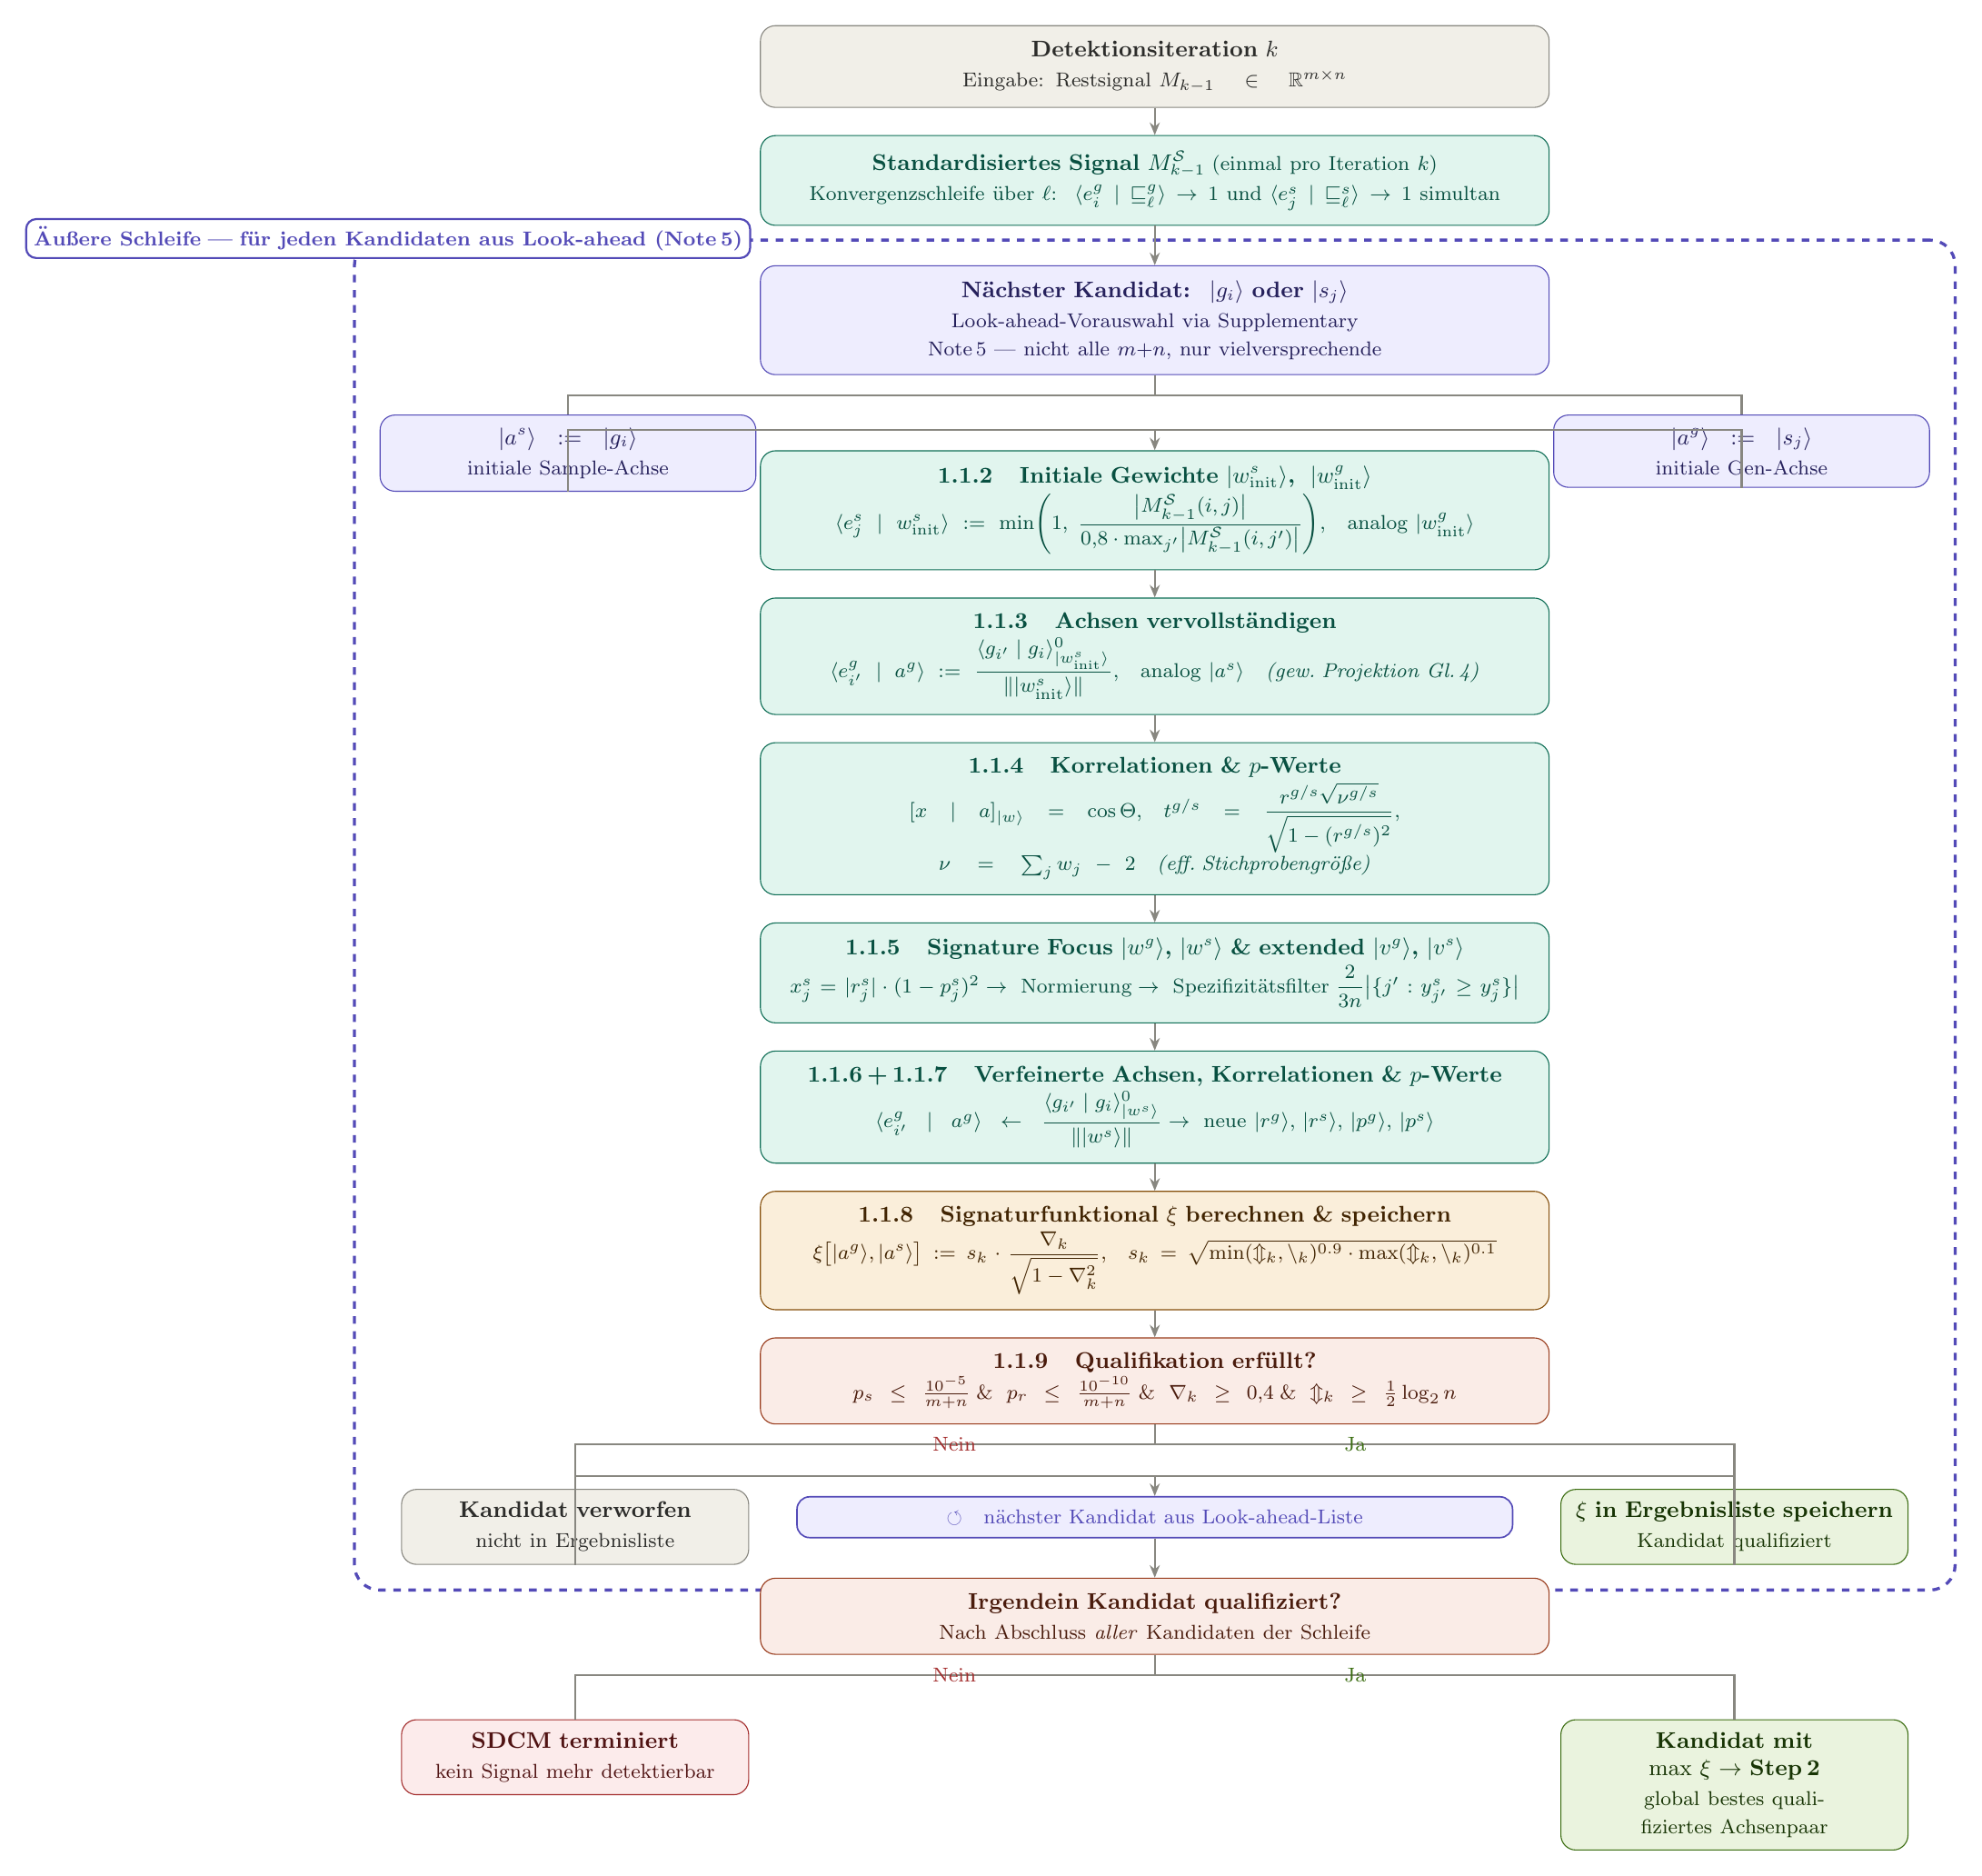
\begin{tikzpicture}[node distance=0.38cm]

% (0) Start
\node[sdcm@gray] (start) {%
  \textbf{Detektionsiteration $k$}\\[1pt]
  {\footnotesize Eingabe: Restsignal $M_{k-1} \in \mathbb{R}^{m \times n}$}%
};

% (1) Standardisierung — once per iteration k, OUTSIDE the loop
\node[sdcm@teal, below=of start] (std) {%
  \textbf{Standardisiertes Signal $M^{\mathcal{S}}_{k-1}$}%
  \;{\footnotesize (einmal pro Iteration $k$)}\\[1pt]
  {\footnotesize Konvergenzschleife über $\ell$:\;
   $\langle e^g_i \mid \mathcal{v}^g_\ell \rangle \to 1$ und
   $\langle e^s_j \mid \mathcal{v}^s_\ell \rangle \to 1$ simultan}%
};

% (2) Candidate — first node inside outer loop
\node[sdcm@purp, below=0.55cm of std] (cand) {%
  \textbf{Nächster Kandidat:\; $|g_i\rangle$ oder $|s_j\rangle$}\\[1pt]
  {\footnotesize Look-ahead-Vorauswahl via Supplementary Note\,5
   — nicht alle $m{+}n$, nur vielversprechende}%
};

% (2a/2b) Branch boxes
\node[sdcm@purpsm, below left=0.55cm and 0.05cm of cand]  (branchL)
  {\textbf{$|a^s\rangle := |g_i\rangle$}\\[1pt]{\footnotesize initiale Sample-Achse}};
\node[sdcm@purpsm, below right=0.55cm and 0.05cm of cand] (branchR)
  {\textbf{$|a^g\rangle := |s_j\rangle$}\\[1pt]{\footnotesize initiale Gen-Achse}};

% (3) Initial weights
\node[sdcm@teal, below=1.05cm of cand] (wini) {%
  \textbf{1.1.2\quad Initiale Gewichte
    $|w^s_\mathrm{init}\rangle$,\; $|w^g_\mathrm{init}\rangle$}\\[1pt]
  {\footnotesize $\displaystyle
    \langle e^s_j \mid w^s_\mathrm{init}\rangle
    := \min\!\left(1,\;
       \frac{\bigl|M^{\mathcal{S}}_{k-1}(i,j)\bigr|}
            {0{,}8\cdot\max_{j'}\bigl|M^{\mathcal{S}}_{k-1}(i,j')\bigr|}
    \right)$,\quad analog $|w^g_\mathrm{init}\rangle$}%
};

% (4) Complete axes
\node[sdcm@teal, below=of wini] (axes) {%
  \textbf{1.1.3\quad Achsen vervollständigen}\\[1pt]
  {\footnotesize $\displaystyle
    \langle e^g_{i'} \mid a^g\rangle
    := \frac{\langle g_{i'} \mid g_i\rangle^0_{|w^s_\mathrm{init}\rangle}}
            {\||w^s_\mathrm{init}\rangle\|}$,\quad
   analog $|a^s\rangle$\quad\textit{(gew.\;Projektion Gl.\,4)}}%
};

% (5) Correlations & p-values
\node[sdcm@teal, below=of axes] (corr) {%
  \textbf{1.1.4\quad Korrelationen \& $p$-Werte}\\[1pt]
  {\footnotesize
   $[x \mid a]_{|w\rangle} = \cos\Theta$,\quad
   $t^{g/s} = \dfrac{r^{g/s}\sqrt{\nu^{g/s}}}{\sqrt{1-(r^{g/s})^2}}$,\quad
   $\nu = \textstyle\sum_j w_j - 2$\quad\textit{(eff.\;Stichprobengröße)}}%
};

% (6) Signature Focus
\node[sdcm@teal, below=of corr] (focus) {%
  \textbf{1.1.5\quad Signature Focus
    $|w^g\rangle$, $|w^s\rangle$ \& extended $|v^g\rangle$, $|v^s\rangle$}\\[1pt]
  {\footnotesize
   $x^s_j = |r^s_j|\cdot(1-p^s_j)^2$\;$\to$\;
   Normierung\;$\to$\;
   Spezifizitätsfilter\;$\dfrac{2}{3n}\bigl|\{j': y^s_{j'}\ge y^s_j\}\bigr|$}%
};

% (7) Refined axes
\node[sdcm@teal, below=of focus] (refit) {%
  \textbf{1.1.6\,+\,1.1.7\quad Verfeinerte Achsen, Korrelationen \& $p$-Werte}\\[1pt]
  {\footnotesize
   $\langle e^g_{i'} \mid a^g\rangle
    \leftarrow \dfrac{\langle g_{i'}\mid g_i\rangle^0_{|w^s\rangle}}
                     {\||w^s\rangle\|}$\;$\to$\;
   neue $|r^g\rangle,\,|r^s\rangle,\,|p^g\rangle,\,|p^s\rangle$}%
};

% (8) Signature functional
\node[sdcm@ambr, below=of refit] (xi) {%
  \textbf{1.1.8\quad Signaturfunktional $\xi$ berechnen \& speichern}\\[1pt]
  {\footnotesize $\displaystyle
    \xi\bigl[|a^g\rangle,|a^s\rangle\bigr]
    := s_k\cdot\frac{\mathcal{r}_k}{\sqrt{1-\mathcal{r}_k^2}}$,\quad
   $s_k=\sqrt{\min(\mathcal{m}_k,\mathcal{n}_k)^{0.9}
               \cdot\max(\mathcal{m}_k,\mathcal{n}_k)^{0.1}}$}%
};

% (9) Qualification
\node[sdcm@corl, below=of xi] (qual) {%
  \textbf{1.1.9\quad Qualifikation erfüllt?}\\[1pt]
  {\footnotesize
   $p_s\le\tfrac{10^{-5}}{m+n}$\;\&\;
   $p_r\le\tfrac{10^{-10}}{m+n}$\;\&\;
   $\mathcal{r}_k\ge0{,}4$\;\&\;
   $\mathcal{m}_k\ge\tfrac{1}{2}\log_2 n$}%
};

% Qualification branch outcomes
\node[sdcm@disc, below left=0.9cm  and 0.15cm of qual] (disc)
  {\textbf{Kandidat verworfen}\\[1pt]{\footnotesize nicht in Ergebnisliste}};
\node[sdcm@gren, below right=0.9cm and 0.15cm of qual] (save)
  {\textbf{$\xi$ in Ergebnisliste speichern}\\[1pt]{\footnotesize Kandidat qualifiziert}};

% Loop-back banner
\node[sdcm@loop, below=1.0cm of qual] (loopback)
  {$\circlearrowleft$\quad nächster Kandidat aus Look-ahead-Liste};

% Final decision (outside loop)
\node[sdcm@corl, below=0.55cm of loopback] (anyq) {%
  \textbf{Irgendein Kandidat qualifiziert?}\\[1pt]
  {\footnotesize Nach Abschluss \emph{aller} Kandidaten der Schleife}%
};

% Final outcomes
\node[sdcm@red,  below left=0.9cm  and 0.15cm of anyq] (term)
  {\textbf{SDCM terminiert}\\[1pt]{\footnotesize kein Signal mehr detektierbar}};
\node[sdcm@gren, below right=0.9cm and 0.15cm of anyq] (step2)
  {\textbf{Kandidat mit $\max\,\xi$ $\to$ Step\,2}\\[1pt]
   {\footnotesize global bestes qualifiziertes Achsenpaar}};

% Outer loop dashed frame
\begin{scope}[on background layer]
  \node[draw=sdcm@purp@bd, line width=1.2pt, dashed, fill=none,
    rounded corners=10pt, inner sep=10pt,
    fit=(cand)(branchL)(branchR)(wini)(axes)(corr)
        (focus)(refit)(xi)(qual)(disc)(save)(loopback)
  ] (outerloop) {};
\end{scope}
\node[fill=white, draw=sdcm@purp@bd, line width=0.8pt, rounded corners=4pt,
  inner sep=3pt, font=\footnotesize\bfseries, text=sdcm@purp@bd
] at (outerloop.north west) [xshift=14pt]
  {Äußere Schleife\;—\;für jeden Kandidaten aus Look-ahead (Note\,5)};

% Arrows
\draw[sdcm@arr]  (start.south) -- (std.north);
\draw[sdcm@arr]  (std.south)   -- (cand.north);

\coordinate (splitPt) at ($(cand.south)+(0,-0.28)$);
\draw[sdcm@line] (cand.south) -- (splitPt);
\draw[sdcm@line] (splitPt) -| (branchL.north);
\draw[sdcm@line] (splitPt) -| (branchR.north);

\coordinate (mergePt) at ($(wini.north)+(0,0.28)$);
\draw[sdcm@line] (branchL.south) |- (mergePt);
\draw[sdcm@line] (branchR.south) |- (mergePt);
\draw[sdcm@arr]  (mergePt) -- (wini.north);

\draw[sdcm@arr] (wini.south)  -- (axes.north);
\draw[sdcm@arr] (axes.south)  -- (corr.north);
\draw[sdcm@arr] (corr.south)  -- (focus.north);
\draw[sdcm@arr] (focus.south) -- (refit.north);
\draw[sdcm@arr] (refit.south) -- (xi.north);
\draw[sdcm@arr] (xi.south)    -- (qual.north);

\coordinate (qSplit) at ($(qual.south)+(0,-0.28)$);
\draw[sdcm@line] (qual.south) -- (qSplit);
\draw[sdcm@line] (qSplit) -| (disc.north);
\draw[sdcm@line] (qSplit) -| (save.north);
\node[font=\footnotesize, text=sdcm@red@bd]  at ($(qSplit)+(-2.8,0)$) {Nein};
\node[font=\footnotesize, text=sdcm@gren@bd] at ($(qSplit)+(+2.8,0)$) {Ja};

\coordinate (lbMerge) at ($(loopback.north)+(0,0.28)$);
\draw[sdcm@line] (disc.south) |- (lbMerge);
\draw[sdcm@line] (save.south) |- (lbMerge);
\draw[sdcm@arr]  (lbMerge)   -- (loopback.north);
\draw[sdcm@arr]  (loopback.south) -- (anyq.north);

\coordinate (aSplit) at ($(anyq.south)+(0,-0.28)$);
\draw[sdcm@line] (anyq.south) -- (aSplit);
\draw[sdcm@line] (aSplit) -| (term.north);
\draw[sdcm@line] (aSplit) -| (step2.north);
\node[font=\footnotesize, text=sdcm@red@bd]  at ($(aSplit)+(-2.8,0)$) {Nein};
\node[font=\footnotesize, text=sdcm@gren@bd] at ($(aSplit)+(+2.8,0)$) {Ja};

\end{tikzpicture}
\end{document}